\documentclass[a4paper, twoside]{report}
%% Language and font encodings
\usepackage[english]{babel}
\usepackage[utf8x]{inputenc}
\usepackage[T1]{fontenc}

%% Chapter Beautify
\usepackage{titlesec}
% \newcommand{\hsp}{\hspace{20pt}}
% \titleformat{\chapter}[hang]{\Huge\bfseries}{\thechapter\hsp|\hsp}{0pt}{\Huge\bfseries}

%% Very nice Font
\usepackage{palatino}

%% Diagram drawing
\usepackage{tikz}
\usetikzlibrary{shapes.geometric, arrows}

%% Forced float
\usepackage{float}

%% Source code highlight
\usepackage{minted}
\usepackage{listings}

%% figure

%% Code line references
\setminted[haskell]{escapeinside=\#\#, linenos=true, mathescape=true}
\usepackage{caption}
\usepackage{tikz}
\newcommand*\circled[1]{\tikz[baseline=(char.base)]{
            \node[shape=circle,draw,inner sep=1pt, text=white] (char) {#1};}}
\newcommand*\clabel[1]{$\label{#1} \circled{\ref{#1}}$}
\newcommand*\cref[1]{\circled{\ref{#1}}}
\newcommand*\ccaption[2]{
    \caption[.]{
        \centering #1\newline
        \begin{minipage}{\linewidth}
            #2
        \end{minipage}
        \newline
    }
}

\newenvironment{code}{\captionsetup{type=listing}}{}
%% Automatic Reference

% BNF Rule
\usepackage{mathtools,array}
\newenvironment{grammar}[2]
 {\begin{tabular}{@{\qquad}>{$}l<{$}@{\qquad}l@{}}
  \multicolumn{1}{@{}l@{}}{$#1$}&\multicolumn{1}{l@{}}{\hspace{-2em}#2}\\}
 {\end{tabular}}

%% Placeholder picture
\usepackage{mwe}

%% Format Paragraph
\setcounter{secnumdepth}{4}
\titleformat{\paragraph}
{\normalfont\normalsize\bfseries}{\theparagraph}{1em}{}
\titlespacing*{\paragraph}
{0pt}{3.25ex plus 1ex minus .2ex}{1.5ex plus .2ex}

%% Sets page size and margins
\usepackage[a4paper,top=3cm,bottom=2cm,left=3cm,right=3cm,marginparwidth=1.75cm]{geometry}

%% Useful packages
\usepackage{amsmath}
\usepackage{amssymb}
\usepackage{graphicx}
\usepackage{subcaption}
\usepackage[colorinlistoftodos]{todonotes}
\usepackage[colorlinks=true, allcolors=black]{hyperref}

%% Reference for figure, section and source code
\newcommand*{\tabref}[1]{\tablename~\ref{#1}}
\newcommand*{\figref}[1]{\figurename~\ref{#1}}
\newcommand*{\coref}[1]{\lstlistingname~\ref{#1}}
\newcommand*{\secref}[1]{Section~\ref{#1}}

%% Line number
% \usepackage{lineno}
% \linenumbers

%% for example
\usepackage{xspace}
\newcommand*{\eg}{e.g.\@\xspace}

%% Nested list
\usepackage{enumitem}
\setlist[enumerate]{label*=\arabic*.}

%% Haskell 
\newcommand*{\hask}[1]{\mintinline{text}{#1}}

%% https://tex.stackexchange.com/questions/375992/bad-mathchar-with-semantic-package
\usepackage{semantic}

\title{TODO}
\author{Shuhao Zhang}
% Update supervisor and other title stuff in title/title.tex

\begin{document}
\begin{titlepage}

\newcommand{\HRule}{\rule{\linewidth}{0.5mm}} % Defines a new command for the horizontal lines, change thickness here

%----------------------------------------------------------------------------------------
%	LOGO SECTION
%----------------------------------------------------------------------------------------


\includegraphics[width=8cm]{title/logo.png}\\[1cm] % Include a department/university logo - this will require the graphicx package
 
%----------------------------------------------------------------------------------------

\center % Center everything on the page

%----------------------------------------------------------------------------------------
%	HEADING SECTIONS
%----------------------------------------------------------------------------------------

\textsc{\LARGE MEng Individual Project}\\[1.5cm] % Name of your university/college
\textsc{\Large Imperial College London}\\[0.5cm] % Major heading such as course name
\textsc{\large Department of Computing}\\[0.5cm] % Minor heading such as course title

%----------------------------------------------------------------------------------------
%	TITLE SECTION
%----------------------------------------------------------------------------------------
\makeatletter
\HRule \\[0.4cm]
{ \huge \bfseries \@title}\\[0.4cm] % Title of your document
\HRule \\[1.5cm]
 
%----------------------------------------------------------------------------------------
%	AUTHOR SECTION
%----------------------------------------------------------------------------------------

\begin{minipage}{0.4\textwidth}
\begin{flushleft} \large
\emph{Author:}\\
\@author % Your name
\end{flushleft}
\end{minipage}
~
\begin{minipage}{0.4\textwidth}
\begin{flushright} \large
\emph{Supervisor:} \\
Prof. Nobuko Yoshida\\[1.2em] % Supervisor's Name
\emph{Second Marker:} \\
TBD
\end{flushright}
\end{minipage}\\[2cm]
\makeatother

% If you don't want a supervisor, uncomment the two lines below and remove the section above
%\Large \emph{Author:}\\
%John \textsc{Smith}\\[3cm] % Your name

%----------------------------------------------------------------------------------------
%	DATE SECTION
%----------------------------------------------------------------------------------------

{\large \today}\\[2cm] % Date, change the \today to a set date if you want to be precise

\vfill % Fill the rest of the page with whitespace

\end{titlepage}

% TODO
% \begin{abstract}
% TBD
% \end{abstract}

% \renewcommand{\abstractname}{Acknowledgements}
% \begin{abstract}
% TBD
% \end{abstract}

\tableofcontents
% \listoffigures
% \listoftables

\chapter{Introduction} \label{chap:intro}
% define the session typed monad language
% Arrow => seesson typed monadic lagnauge
% Turning data flow into communication 
% compile session-typed monadic language to C
% results => a standalone framework for parallel computation
% high-level arrow code => 1) abstraction layer on top of settiontype language  2) a set of local types to reason so that it's possible reason about the structure of parallel computation 
% as a use case => compile to c
% as a use case => backend for ParAlg
% put the picture in the introduction
% 
% title : session-arrow =>  

\section{Motivation} \label{i:m}
Writing parallel software is not a trivial task. Parallel code is hard to write because it is usually written in low level languages with verbose and non-idiomatic decorations, hard to debug because machines, where code is written, are usually different from machines where code is intended to run and hard to maintain and reuse because even though the underlying algorithms are not changed, multiple version of parallel code is needed to tackle various platform and evolution of architectures.

There are many on-going pieces of research aimed at helping programmers write correct parallel programs smoothly. A common approach is to develop a higher level language and compiles programmes in this language to required parallel code. There are many high-level frameworks for parallel programming (\eg algorithmic skeletons\cite{coleAlgorithmicSkeletonsStructured}, domain-specific languages for parallelism\cite{brownHeterogeneousParallelFramework2011} or famous MapReduce parallel model\cite{liMapReduceParallelProgramming2016}). An example is to use arrow terms (\secref{b:arrows}) to describe data flow implicitly and hence generate parallel code.

The workflow of writing parallel code has evolved from writing it directly in the target platform to writing software in a high-level language designed for parallel computation and then compiling to the target platform. In this project, we present a method to improve the backend of parallel code generation by introducing a monadic domain-specific language to act as a bridge between high-level and target low-level parallel languages.

This specific language needs to be general enough so that it supports multiple high-level parallel programming frameworks. It can be used to generate different parallel code, e.g. MPI \footnote{Message Passing Interface (MPI) is a standardized and portable message-passing standard designed by a group of researchers from academia and industry to function on a wide variety of parallel computing architectures \cite{MessagePassingInterface2018}.}, Cuda. Moreover, it can be interpreted with a simulator to aid debugging parallel programs.

% With the help of this intermediate languages, the implementation complexity is reduced from $O(M \times N)$, where each of the M high-level languages needs to implement N compilers to generate parallel code in N different platforms, to $O(M + N)$, where each compiler of a high-level language implements a translation rule to the intermediate language which implements one compiler and N backend to generate different target languages.

In addition, it couples with multiparty session type (MPST) \cite{coppoGentleIntroductionMultiparty2015}. It takes advantages of properties of MPST to enable aggressive optimisation but ensuring code correctness and allow more meaningful static analysis; \eg cost modelling for parallel programming. % (TODO add more examples of possible kinds of static analysis and reference paper).
\section{Contributions} 
\begin{figure}[ht]
    \centering
    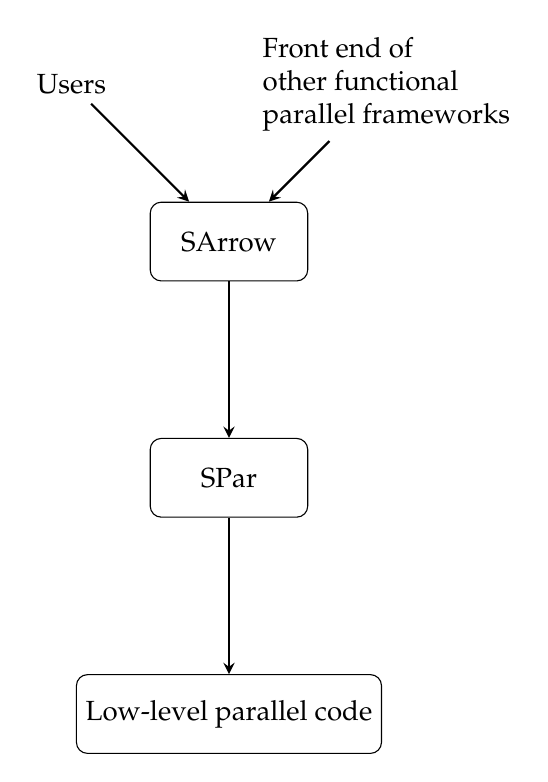
\begin{tikzpicture}[xscale=.5]
    \tikzstyle{proc}  = [rectangle, rounded corners, minimum width=2cm, minimum height=1cm,text centered, draw=black] 
    \tikzstyle{proc1} = [circle,  minimum width=1cm, minimum height=1cm,text centered, draw=black] 
    \tikzstyle{arrow} = [thick,->,>=stealth]
    \node (a) [proc] at (0, 3)  {SArrow};
    \node (b) [proc] at (0, 0)  {SPar};
    \node (c) [proc] at (0, -3) {Low-level parallel code};
    \node (d)  at (-4, 5) {Users};
    \node (e) [align=left] at (4, 5) {Front end of \\ other functional  \\ parallel frameworks};
    \draw[arrow] (a) to (b);
    \draw[arrow] (b) to (c);
    \draw[arrow] (d) to (a);
    \draw[arrow] (e) to (a);
    \end{tikzpicture}
    \caption{Visualization of the workflow}
    \label{intro:fig:workflow}
\end{figure}
The result of project is a embedded high-level framework in Haskell that is capable of generating low-level parallel code. The major contributions are:
\begin{enumerate}
    \item \textbf{Session-typed intermediate language. } We create an intermediate embedded domain specific language (EDSL): SPar: a session typed free monad EDSL for message passing concurrency. This language can be typed by local types, and hence, we can apply multiple results from the multiparty session types to our framework, especially in terms of safety of generated code and reasoning of communication patterns.
    \item \textbf{Intuitive user interface. } One innovation of this project is that we apply the mature Arrow interface for users to express parallel computations. We call the interface SArrow: an arrow interface for writing SPar expressions. It is an abstraction layer on top of SPar, which hides communication primitives from users so that users can express parallel algorithms similar to what they would write for sequential programs.
    \item \textbf{Multiple backends. } We create a backend to generate parallel C code from SPar expressions. The core of the backend is Instr: a low-level EDSL that is independent of target languages. This means that we can support multiple target languages with ease without re-implementing multiple backends. In addition to the code generation backend, we implement an interpreter backend in Haskell for experimenting and fast verification.
    \item \textbf{Evaluations. } Finally, we show the expressive power of the framework by implementing several common computation patterns and three algorithms using our interface. We evaluate the performance of the generated code from the algorithms on high-performance computers as well as PCs. 
\end{enumerate}
The \figref{intro:fig:workflow} summaries the workflow of the framework visually. The main principle supporting the framework is that we convert data flow into communications and from the communication patterns, we gain parallel codes. The results of expressing computation in the framework are 1) compilation to efficient deadlock-free low-level parallel programs and 2) a set of local types to reason the structure of the parallel computation.

At the end of the project, we have discovered two use case of the framework. The primary application is a stand-alone tool to generate parallel C code, and another is a backend for other data-flow based parallel frameworks. 

\section{Report outlines}

\charef{chap:b} gives an overview of the background and related researches. We present the syntax and semantics of SPar in \charef{chap:spar} followed by \charef{chap:impl} introducing the implementation aspect of SPar like session typing and interpreter. \charef{chap:arrow} demonstrates the Arrow interface with examples of parallel patterns formed by the interface and justification of the interface satisfying arrow laws. The discussion about some implementation specific issues like role allocation is also contained in \charef{chap:arrow}. In \charef{chap:cg}, we show the code generation backend and discuss our solutions to challenges when compiling to C, i.e. the problem of representing polymorphic algebraic data structure in C. \charef{chap:eval} explains our benchmarks and shows the performance of the generated code. This chapter can also be regarded as a tutorial on how to use the framework. Finally, we conclude with potential future improvements and remarks on this project. We also include the generated C code in the appendix for curious readers.
\chapter{Background} \label{b}
% This section is an overview of arrows, multiparty session types (MPST) and free monad. Arrow is an interface of implicit data flow, and MPST can be used to describe explicit data flow. Free monad is a technique to convert normal DSL to a monadic DSL. 
% As mentioned in the \secref{i:m}, this section is an overview of a high-level language (\secref{b:arrows} and \secref{b:pal}), from which a translation rule will be proposed to our intermediate languages, multiparty session types (\secref{b:mpst}), the theoretical backbone giving rich features of the intermediate languages, and the free monad (\secref{b:fm}), a technique in designing the intermediate languages.
This section is an overview of techniques that influence the design choices of our monadic language for parallel computation. First of all, we give an overview of techniques applied in the high-level parallel programming framework: arrows (\secref{b:arrows}) and recursion schemes (\secref{b:rs}). We then introduce several techniques for message-passing concurrency: multiparty session types (\secref{b:mpst}) and monadic languages for concurrency (\secref{b:mo}). In the end, we introduce free monads (\secref{b:fm}), a technique valuable in implementing embedded domain-specific languages (EDSL).

\section{Arrows} \label{b:arrows}
Arrow is a general interface to describe computation. It can ease the process of writing structured code suitable for parallelising. It also demos a common feature of the frameworks: parallelizability is empowered by underlying implicit but precise data-flow. On the other hand, converting to low-level message-passing code, which requires programmers to define communication using message-passing function and primitives, makes the data-flow explicit.
\subsection{Definition}
\coref{b:ar:c1} shows the Arrow definition in Haskell. Intuitively, an arrow type \hask{y a b}(that is, the application of the parameterised type \hask{y} to the two parameter types \hask{b} and \hask{c}) can be regarded as a computation with input of type \hask{b} and output of type \hask{b}\cite{hughesGeneralisingMonadsArrows2000}. Visually, arrows are like pipelines (shown in \figref{b:ar:p1}). In Haskell, an arrow \hask{y} is a type that implements the following interface (type classes in Haskell are roughly interfaces). \hask{arr} converts an arbitrary function into an arrow. \hask{>>>} sequences two arrows (illustrated in \figref{b:ar:seq}). Taking two input,  \hask{first} apply the arrow to the first input while keeping the second untouched (\figref{b:ar:first}). Conversely, \hask{second} modifies the second input and keeps the first one unchanged. \hask{***} applies two arrows to two input side by side (\figref{b:ar:par}). \hask{&&&} takes one input and applies two separate arrows to the input and its duplications (\figref{b:ar:dup}).
% TODO add reference to arrow visualization

The simplest instance of arrow class is the function type (shown in \coref{b:ar:c2}). It is worth noticing that only \hask{arr} and \hask{***} need to be implemented. The reset of function in the arrow type class can be defined in terms of the two functions. For example, \mintinline{text}{f &&& g = (f *** g) . arr (\b -> (b, b))} and \mintinline{text}{first = (*** id)}
\begin{code}
  % \inputminted{haskell}{background/ar-def.hs}
  \begin{minted}{haskell}
    class Arrow y where 
      arr :: (a -> b) -> y a b
      first :: y a b -> y (a, c) (b, c)
      second :: y a b -> y (c, a) (c, b)
      (***) :: y a c -> y b d -> y (a, b) (c, d)
      (&&&) :: y a b -> y a c -> y a (b, c)
  \end{minted}
  \caption{Arrow class in Haskell}
  % \ccaption{Arrow class in Haskell}{
    % \begin{itemize}
      % \item[\cref{ar-def:1}] Types of arrow functions 
    % \end{itemize}
  % }
  \label{b:ar:c1}
\end{code}
\begin{code}
  % \inputminted{haskell}{background/ar-func.hs}
  \begin{minted}{haskell}
    instance Arrow (->) where
      arr f = f
      (***) f g ~(x,y) = (f x, g y)
  \end{minted}
  \caption{$(\rightarrow)$ instance of Arrow class}
  \label{b:ar:c2}
\end{code}
\begin{figure*}
  \centering
  \begin{subfigure}[b]{0.475\textwidth}
      \centering
      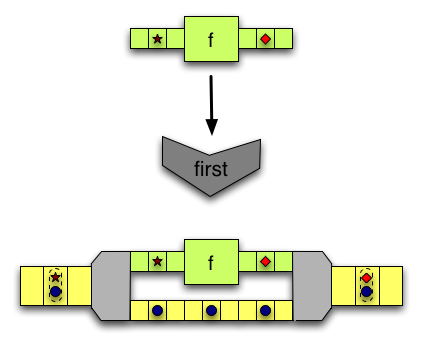
\includegraphics[width=\textwidth]{background/image/ArrowsConveyors_first2.png}
      \caption{\hask{first}}
      \label{b:ar:first}
  \end{subfigure}
  \hfill
  \begin{subfigure}[b]{0.475\textwidth}  
      \centering 
      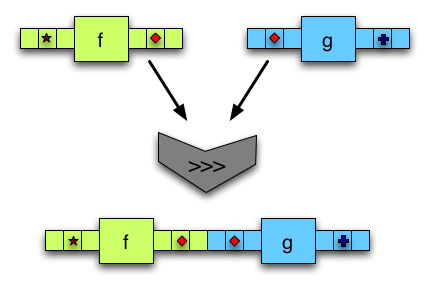
\includegraphics[width=\textwidth]{background/image/ArrowsConveyors_bind2.png}
      \caption{\hask{>>>}}
      \label{b:ar:seq}
  \end{subfigure}
  \vskip\baselineskip
  \begin{subfigure}[b]{0.475\textwidth}   
      \centering 
      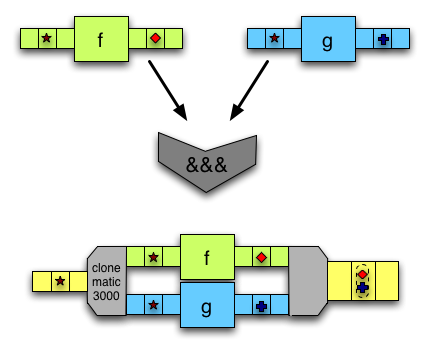
\includegraphics[width=\textwidth]{background/image/ArrowsConveyors_ampersand2.png}
      \caption{\hask{&&&}}
      \label{b:ar:dup}
  \end{subfigure}
  \quad
  \begin{subfigure}[b]{0.475\textwidth}   
      \centering 
      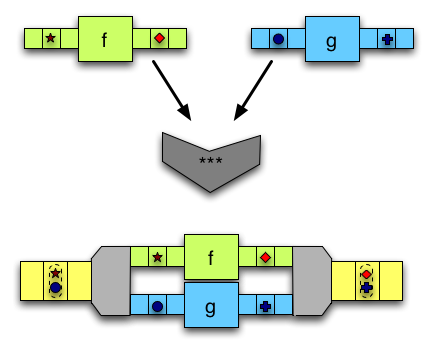
\includegraphics[width=\textwidth]{background/image/ArrowsConveyors_star2.png}
      \caption{\hask{***}}
      \label{b:ar:par}
  \end{subfigure}
  \caption
  {\small The visual representations of arrow combinators\cite{HaskellUnderstandingArrows}}
  \label{b:ar:p1}
\end{figure*}
\subsection{Example: Calculate the mean}
Consider the a function to calculate the mean from a list of floating number, we will compare the usual, arrows implementations. Implementation using arrows can be regarded as point-free programming. Point-free programming is programming paradigm where function definitions only involve combinators and function composition without mentioning variables\cite{TacitProgramming2019}. 

\begin{minted}{haskell}
mean :: [Float] -> Float
mean xs = sum xs / (fromIntegral . length) xs

mean' :: [Float] -> Float
mean' = (sum &&& (length >>> fromIntegral)) >>> uncurry (/)
\end{minted}
The arrows implementation can be visualised in \figref{b:ar:p2}.
\begin{figure}[!ht]
  \centering
  % \includegraphics[width=8cm]{example-image} 
  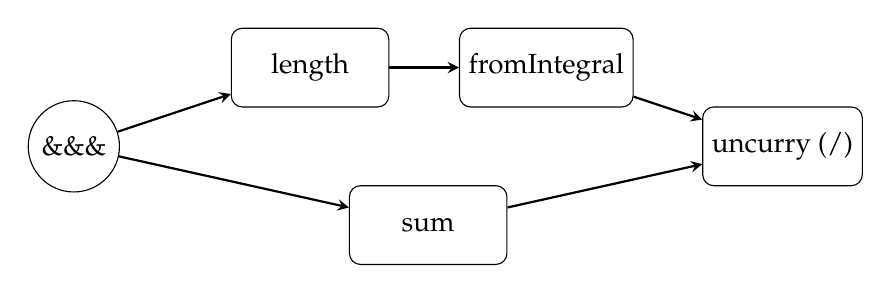
\begin{tikzpicture}[xscale=1.5]
    \tikzstyle{proc} = [rectangle, rounded corners, minimum width=2cm, minimum height=1cm,text centered, draw=black] 
    \tikzstyle{proc1} = [circle,  minimum width=1cm, minimum height=1cm,text centered, draw=black] 
    \tikzstyle{arrow} = [thick,->,>=stealth]
    \node (a) [proc1] at (0, 0) {\&\&\&};
    \node (b) [proc] at (2, 1) {length};
    \node (c) [proc] at (4, 1) {fromIntegral};
    \node (d) [proc] at (6, 0) {uncurry (/)};
    \node (e) [proc] at (3, -1) {sum};
    \draw[arrow] (a) to (b);
    \draw[arrow] (b) to (c);
    \draw[arrow] (c) to (d);
    \draw[arrow] (a) to (e);
    \draw[arrow] (e) to (d);
  \end{tikzpicture}
  \caption{Visualization of mean'}\label{b:ar:p2}
\end{figure}
\begin{minted}{haskell}
mean'' :: [Float] -> Float
mean'' = liftM2 (/) sum (fromIntegral . length)
\end{minted}
Arrows are not the only way to form point-free programs. The above code snippet is the more traditional approach form of point-free mean function in Haskell. We can argue this form of point-free function is more difficult to understand compared to arrows because it involves knowledge of monads (\hask{liftM2}) and does not map to intuitive data-flow.

The simple example demos that arrows combinators make writing point-free programs easier. Arrows union the implementation of algorithm and data-flow in the algorithm. 

\subsection{Application in parallel computation}
From the previous example, the data flow of programs written regarding arrow combinators can be easily visualised (shown in \figref{b:ar:p1}). It is intuitive to recognise that the clean separation between the flow of data and actual computation will be useful in generating parallel code. Indeed, arrow describes data flow implicitly, and it is an example of the so-called algebraic pattern. Many works \cite{braunArrowsParallelComputation2018, elliottGenericFunctionalParallel2017b, AlgebraicMultipartyProtocol} has been done to generate parallel code from algebraic patterns.
In particular, details of \cite{AlgebraicMultipartyProtocol} are introduced in later section. % TODO

\section{Recursion Schemes} \label{b:rs}
Recursion schemes are patterns for expressing general computation. In particular, they are like high order function abstracting recursion so that programmer can express any kind of recursion by data structures combined with recursion schemes instead of writing explicit recursive functions.
\subsection{Definition}
We will introduce three typical recursion schemes: catamorphisms, anamorphisms and hylomorphisms (seen in \coref{p:pal:c3}). As mentioned before, recursion schemes express recursion with the help of data structures, in particular, the fixed point of data structures (seen in \coref{p:pal:c2})
\begin{code}
\begin{minted}{haskell}
newtype Fix f = Fix { unfix :: f (Fix f) }

data TreeF a =
    Node a a
  | Leaf int
  | Empty
  deriving Functor

type Tree = Fix TreeF
\end{minted}
\caption{Definition of fix point of data structures} \label{p:pal:c2}
\end{code}

Anamorphisms takes a function from a to f a (called the co-algebra) and a value a and return the Fix f. Used Tree as an example, anamorphisms takes a single value a and applies the co-algebra to the value. It continues to apply itself to the branches of the TreeF recursively and finally expands a single value to a complete tree. Intuitively, anamorphism unfolds a single value to a complicated data structure top-down.

Catamorphisms is the reverse of anamorphisms, folding a data structure to a single value bottom-up. It takes a function from f a to a (called the algebra) and Fix f to fold and return a single value a. Catamorphisms and anamorphisms describe the process globally (from a to Fix f and from Fix f to a) while co-algebra and algebra capture what happened locally. The elegant part is while co-algebra and algebra do not involve with any recursion data structure (TreeF is not recursive), catamorphisms consumes recursive data structure while anamorphism builds them.

Hylomorphisms applies anamorphism followed by catamorphisms. It is the most common pattern to use. We will use an example to illustrate its usefulness. It can be thought of as an abstract divide and conquer algorithm.
% TODO add Divided and conquer analogy
\begin{code}
\begin{minted}{haskell}
ana :: Functor f => (a -> f a) -> a -> Fix f
ana coalg = Fix . fmap (ana coalg) . coalg

cata :: Functor f => (f a -> a) -> Fix f -> a
cata alg = alg . fmap (cata alg) . unfix

hylo :: (f b -> b) -> (a -> f a) -> b -> a 
hylo g f = f . fmap (hylo f g) . g
\end{minted}
\caption{Recursion schemes in haskell} \label{p:pal:c3}
\end{code}

\subsection{Example: Merge sort} \label{b:rs:ex}
We can write merge sort recursively. First of all, we split the list in half and then apply the merge sort recursively to both parts and finally we merge two lists into a single list. 

To write merge sort in terms of recursion scheme, we need to define the recursive structure to represent the control structure. By the definition of merge sort, this structure must have a case with two branches, a base case representing a singleton list and a base case representing an empty list hence this structure is the TreeF we defined above. Splitting a list is like co-algebra while merging is like algebra. We use hylomorphisms to combine them hence getting a sorted list (seen in \coref{p:pal:c4}).
\begin{code}
\inputminted{haskell}{project/pal-ms.hs}
\caption{Merge sort using hylomorphisms} \label{p:pal:c4}
\end{code}
\section{Multiparty session types} \label{b:mpst}
In complicated distributed systems, participants agree on a protocol, specifying type and direction of data exchanged. Multiparty session types are a branch of behavioural types specifically targeted at describing protocols in distributed systems based on asynchronous communication \cite{coppoGentleIntroductionMultiparty2015}. They are a type formalism used to model communication-based programming by codifying the structure of communication. The evolution of computing from the era of data processing to the era of communication witnessed the growth and significance of the theory of session types.

The theory of multiparty session type contains three main elements. Global types (seen in \secref{b:mpst:st}), local (session) types and processes. Processes are the concrete descriptions of the behaviour of the peers involved in the distributed system \cite{coppoGentleIntroductionMultiparty2015} using a formal language. Usually, the most used and the original language is $\pi$-calculus \cite{milnerCalculusMobileProcesses1992}.  However, for the simplicity, we will not introduce $\pi$-calculus % and use message passing primitives in Haskell (seen in section \label{b:mo:mpc}) instead. 
The coming sections are an intuitive introduction of session types by examples.
% TODO: Add descriptions about the MPST 1. describes explicit dataflow 2. so it can be used as the high-level programming languages to generate parallel code 3. in \secref{b:mpst:app}.
\subsection{Global types and local types} \label{b:mpst:st}
Global type is at the most abstract level, describing a communication protocol from a neutral viewpoint between two or more participants\cite{coppoGentleIntroductionMultiparty2015}. The syntax of the global types is shown in \tabref{b:mpst:gt} and an example of global types is shown in \tabref{b:mpst:gtex}.

Local types or session types characterise the same communication protocol as the global type, but from the viewpoint of each peer \cite{coppoGentleIntroductionMultiparty2015}. Each process is typed by local type. The syntax of local types is shown in \tabref{b:mpst:lt} and an example of local type is shown in \tabref{b:mpst:ltex}. 

The relationship between global types and local types are established by the projection operator (seen in the \secref{b:mpst:proj}), and a type system performs syntactic checks, ensuring that processes are typed by their corresponding local types. Hence, at the compile time, three important properties follow \cite{coppoGentleIntroductionMultiparty2015}. 
\begin{itemize}
  \item \textbf{communication safety}: Mismatches between the types of sent and expected messages, despite the same communication channel is used for exchanging messages of different types, do not exist \cite{coppoGentleIntroductionMultiparty2015}. 
  \item \textbf{protocol fidelity}: The interactions that occur are accounted for by the global type and therefore are allowed by the protocol \cite{coppoGentleIntroductionMultiparty2015}.
  \item \textbf{progress}: Every message sent is eventually received, and every process waiting for a message eventually receives one \cite{coppoGentleIntroductionMultiparty2015}.
\end{itemize}
We will learn that these properties are valuable not only in the distributed system but also in the domain of parallel computing in \secref{b:mpst:app}.
% In the theory of multiparty session types, the whole distributed system is described by global types representing the communication protocols from a global viewpoint.  Each process is typed by local types which characterise the same communication protocols as global types but from a perspective of individual participants \cite{coppoGentleIntroductionMultiparty2015}.
\begin{table}[ht]
\centering
\begin{grammar}{G\Coloneqq}{Global types}
  p \rightarrow q : \langle S \rangle.G & Value exchange \\
  p \rightarrow q : \langle T \rangle.G & Channel exchange \\
  p \rightarrow q : \{ l_i : G_i \}_{i \in I} & Bracnhing \\
  \mu \mathbf{t}.G  \mid \mathbf{t} \mid \text{end} & Recursion/End
\end{grammar}
\caption{Global types} \label{b:mpst:gt}
\end{table}
\begin{table}[ht]
\begin{grammar}{S\Coloneqq}{Sorts}
  \text{bool} \mid \text{nat} \mid \text{string} \\
  \dots\\
\end{grammar}
\hfill
\begin{grammar}{T\Coloneqq}{Session types/local types}
  ! \langle p, S \rangle . T & Send value\\
  ! \langle p, T \rangle . T & Send channel\\
  ? ( p, T ) . T & Channel Receive\\
  ? ( p, S ) . T & Sorts Receive\\
  \oplus \langle p, \{ l_i : T_i \}_{i \in I} \rangle & Selection \\
  \&(p, \{l_i : T_i \}_{i \in I}) & Bracnhing \\
  \mu \mathbf{t}.T  \mid \mathbf{t} \mid \text{end} & Recursion/End
\end{grammar}
\caption{Session types/local types} \label{b:mpst:lt}
\end{table}
\begin{table}[ht]
  \begin{minipage}{0.45\textwidth}
    \begin{enumerate}
      \item Customer(0) sends an order number to Agency(1), and Agency sends back a quote to the customer.
      \item If Customer is happy with the price then Customer selects accept option and notifies Agency.
      \item If Customer thinks the price is too high then Customer terminate the trade by selecting reject.
      \item If accept is selected, Agency notify both Customer and Agency2(2). 
      \item Customer sends an address to Agency2 and Agency2 sends back a delivery date.
    \end{enumerate}
  \end{minipage}
  \hfill
  \begin{minipage}{0.45\textwidth}
    \begin{align*}
      G = \\
      & 0 \rightarrow 1: && \langle \text{string} \rangle .\\
      & 1 \rightarrow 0: && \langle \text{int} \rangle .\\
      & 0 \rightarrow 1: \{ && \text{accept}: \\
      & && 1 \rightarrow \{ 0, 2 \}: \langle \text{string} \rangle . \\
      & &&  0 \rightarrow 2: \langle \text{string} \rangle .\\
      & &&  2 \rightarrow 0: \langle \text{int} \rangle . \text{end}, \\
      & && \text{reject}: \text{end} \} \\
    \end{align*}
  \end{minipage}
  \caption{An example of a protocal described by global types G}
  \label{b:mpst:gtex}
\end{table}
\begin{table}[ht]
  \begin{minipage}{0.45\textwidth}
    \begin{align*}
      S \triangleq \mu t.(\&\{ & \text{balance}: ![\text{nat}];t, \\
        & \text{deposit}: ?[\text{nat}];![\text{nat}];t, \\
        & \text{exit}: \text{end}\}) \\
    \end{align*}
  \end{minipage}
  \hfill
  \begin{minipage}{0.45\textwidth}
    \begin{align*}
      C \triangleq \oplus \{ &\text{balance}: ?[\text{nat}];\text{end}, \\
                             &\text{deposit}: ![\text{nat}];?[\text{nat}];\text{end} \} 
    \end{align*}
  \end{minipage}
  \caption{Session types of client and server end point of a ATM service}
  \label{b:mpst:ltex}
\end{table}
\subsubsection{Projection between global types and local types} \label{b:mpst:proj}
Projection is the formalisation of the relationship between global and local types. It is an operation extracting the local type of each peer from the global type \cite{coppoGentleIntroductionMultiparty2015}. The definition of projection is shown in \tabref{b:mpst:pdef}.

As an example, a projection of global type in \tabref{b:mpst:gtex} is
$$
  G \upharpoonright 0 = !\langle 1, \text{string} \rangle;?(1, \text{string});\&(1, \{ \text{accept}: ?(1, \text{string});!\langle 2, \text{string} \rangle;?(2, \text{int}), 
  \text{reject}: \text{end} \})
$$  
\begin{table}[H]
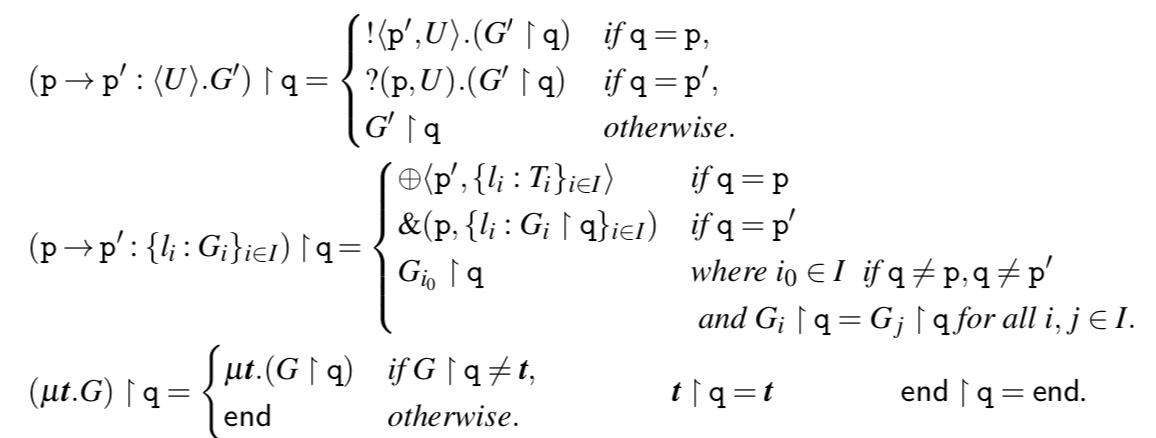
\includegraphics[width=\textwidth]{background/image/proj-def.png}
\caption{The definition of projection of a global type G onto a participants q\cite{coppoGentleIntroductionMultiparty2015}}
\label{b:mpst:pdef}
\end{table}
\subsubsection{Duality of session types}
In binary session types where all protocals are pairwise, duality formalises the relationship between the types of opposite endpoints. For a type $T$, its dual or co type, written $\bar{T}$ is defined inductively as in \tabref{b:mpst:dualdef}.
\begin{table}[H]
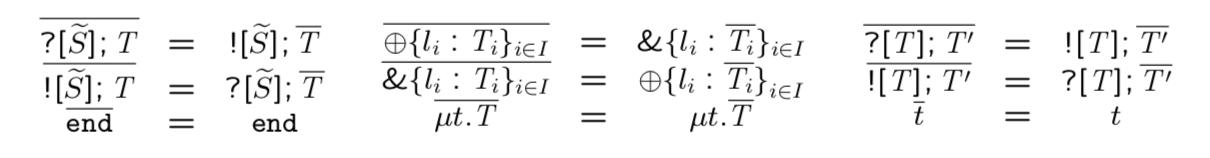
\includegraphics[width=\textwidth]{background/image/dual-def.png}
\caption{Inductive definition of duality}
\label{b:mpst:dualdef}
\end{table}

Duality is essential for checking type compatibility. Compatible types mean that each common channel $k$ is associated with complementary behaviour: this ensures that the interactions on $k$ run without errors. 

In order to apply duality into multiparty session types in which more than two participants are allowed, the partial projection operation (seen in \cite{coppoGentleIntroductionMultiparty2015}) from multiparty session type to binary session type was introduced to allow reusing the definition of duality after applying the partial projection.
% \begin{table}[H]
% \caption{The pa}
% \label{b:mpst:partproj}
% \end{table}
% \begin{table}[ht]
% \begin{align*}
% \end{align*}
% \caption{Inductive definition of duality} \label{b:mpst:dual}
% \end{table}
% \subsection{Example: arithmetic server}
\subsection{Applications in parallel computing} \label{b:mpst:app}
Multiparty session types not only have rich applications in distributed systems but also value in the domain of parallel computation. 

Existing work\cite{ngSafeMPICode} has shown how to generate MPI\footnote{Message Passing Interface (MPI) is a standardised and portable message-passing standard designed by a group of researchers from academia and industry to function on a wide variety of parallel computing architectures \cite{MessagePassingInterface2018}.} programs using session types. Users describe the communication topology as a skeleton using a protocol language which is type checked by session types. After that, an MPI program is generated by merging the skeleton and user-provided kernels for each peer. The parallel code obtained in this way is guaranteed to be deadlock-free and progressing. 

\section{Message passing concurrency} \label{b:mo}
This section introduces some interfaces for message passing concurrency from the primitive case: channel to more advanced one: monad for message passing concurrency.

For simplicity, they are represented in Haskell, but in general, most languages can implement similar interfaces. 
\subsection{Primitives for message-passing concurrency} \label{b:mo:mpc}
In \secref{b:mpst}, channels are bi-directional and used for communication between two parties. In Haskell, channel primitives are represented in \coref{b:mo:c1}. However, just using these primitives cannot guarantee progress or communication safety. For example, a program that has one thread writing channel once combined with another thread reading channel twice is type-correct but will cause deadlock. Many kinds of research to encode MPST using Haskell's type system are presented in \cite{orchardSessionTypesLinearity} so that an (MPST) type-correct Haskell program assures progress, communication safety and session fidelity.
\begin{listing}[ht]
  \inputminted{haskell}{background/mo-chan.hs}
  \caption{Channel primitives in Haskell}
  \label{b:mo:c1}
\end{listing}
\subsection{Concurrency Monads}
The work done by \cite{claessenFunctionalPearlsPoor1999} constructs a monad to express concurrent computation. The definition is in \coref{b:mo:def}. \hask{Action} is the algebraic datatype representing basic concurrency primitives. \hask{Atom}, the atomic unit of computation, is a computation (wrapped in the \hask{IO} monad) followed by an action. \hask{Fork} is two parallel action. \hask{Stop} is the termination of an action. type \hask{C} is a special case of the continuation monad. The continuation monad is an encapsulation of computations in continuation-passing style (CPS)\footnote{In continuation-passing style function result is not returned, but instead is passed to another function, received as a parameter (continuation)\cite{ControlMonadCont}}. SO \hask{C a} is a CPS computation that produces an intermediate result of type \hask{a} within a CPS computation whose final result type is \hask{Action}. With the help of the monad \hask{C}, sequencing and composing actions can use monadic bind.
\begin{code}
  \begin{minted}{haskell}
data Action =
    Atom (IO Action)
  | Fork Action Action
  | Stop

newtype C a = C { runC :: (a -> Action) -> Action } #\clabel{mo-cm:5}#
    
instance Monad C where
    (>>=) :: C a -> (a -> C b) -> C b #\clabel{mo-cm:6}#
    m >>= f  = C $ \k -> runC m (\v -> runC (f v) k)
    return :: a -> C a
    return x = C $ \k -> k x
  \end{minted}
  \caption{The definition of concurrency monad}
  \label{b:mo:def}
\end{code}


The idea is using continuation to represent the "future" so that computation can pause and resume as well as expressing sequential computation. Atom wraps the actual computation and Fork is responsible for spawning threads. In addition, in order to write programmes in a monadic way easier, some helper functions are defined (shown in \coref{b:mo:helper}). \hask{atom} lifts an IO computation to \hask{C}. And \hask{fork} takes a computation in \hask{C} and return a \hask{C} which involves the \hask{Fork} action. Given a \hask{C a}, \hask{action} gives the result of running the CPS computation. We use \hask{\_. Stop} to represent the final continuation (\hask{Stop} action is the last action). 
\begin{code}
\begin{minted}{haskell}
atom :: IO a -> C a
atom m = C $ \k -> Atom $ do
    r <- m
    return $ k r

fork :: C () -> C ()
fork m = C $ \k -> Fork (runC m (const Stop)) (k ())

action :: C a -> Action
action m = m (\_. Stop)
\end{minted}
\caption{Helper functions}
\label{b:mo:helper}
\end{code}
An example of programme written in the concurrency monad is shown below.
\begin{code}
  \begin{minted}{haskell}
example :: C ()
example = do 
  atom $ putStrLn "Hello" 
  name <- atom getLine 
  fork $ atom $ putStrLn "World"
  atom $ putStrLn name
  \end{minted}
\end{code}
We can easily define a round-robin scheduler for programmes in this monad. We can regard a list of action as a queue of threads that are running concurrently. \hask{schedule} will pattern match on the head of the list. If it is \hask{Atom} then the scheduler will run the computation (seen \hask{a <- ioa} at \cref{mo-cm:1}) and pause its remaining computation and put it at the end of the thread queue (seen at \cref{mo-cm:2}). If it is \hask{Fork} then the scheduler will spawn the thread and put the new thread and the current thread to the bottom of the queue (seen at \cref{mo-cm:3}). Finally, If it is \hask{Stop} then it means this thread has finished and the scheduler will resume with the rest of threads in the queue. For example, to run the above example, we call \hask{schedule [action example]}.
\begin{code}
  \begin{minted}{haskell}
schedule :: [Action] -> IO () 
schedule [] = return ()
schedule (a:as) = sched as a
    
sched :: [Action] -> Action -> IO ()
sched as (Atom ioa) = do
    a <- ioa #\clabel{mo-cm:1}#
    schedule $ as ++ [a] #\clabel{mo-cm:2}#
sched as (Fork a1 a2) = schedule $ as ++ [a2, a1] #\clabel{mo-cm:3}#
sched as Stop = schedule as
  \end{minted}
\end{code}

The concurrency monad can be extended to support many features. For example, work done by \cite{marlowMonadDeterministicParallelism} modifies the definition of Action as well as implements a work-stealing parallel scheduler (seen in \coref{b:mo:c3}) to build a monad for parallel computation. 

Besides, extending the concurrency monad to monad for message-passing concurrency can be done by adding channel primitives like newChan, writeChan and readChan into the Action. Since channel primitives are possible to represent in this monad, we naturally think of its prospect in connecting with MPST (will be discussed in the later section).
\begin{code}
  % \inputminted{haskell}{background/mo-par.hs}
  \begin{minted}{haskell}
newtype IVar a = IVar (IORef (IVarContents a)) #\clabel{po:ivar}#
data IVarContents a = Full a | Blocked [a -> Action.]
    
data Action .=
    Fork Action Action
  | Stop
  | forall a . Get (IVar a) (a -> Action) #\clabel{po:get}#
  | forall a . Put (IVar a) a Action #\clabel{po:put}#
  | forall a . New (IVar a -> Action)
  \end{minted}
  \ccaption{Par Monad}{
    \begin{itemize}
      \item[\cref{po:ivar}] Parent threads and child threads communicate data via IVar
      \item[\cref{po:get}] Get operation blocks when the underlying IVarContents is Blocked  
      \item[\cref{po:put}] Put operation updates the underlying IVarContetns to Full with the result a and resume the list of blocking threads by applying a to the continuation.
    \end{itemize}
  }
  \label{b:mo:c3}
\end{code}

In summary, many techniques and ideas like continuation presented in the implementation of this monad afford us inspirations in designing our intermediate language.
\section{Free monad} \label{b:fm}
% TODO add reference to the concurrency monad, show that monad C is not necessary
Free monad\cite{contributorsCatsFreeMonads} is a concept from category theory. Intuitively, a free monad as a programming abstraction is a technique for implementing EDSLs, where a functor represents basic actions of the EDSL and the free monad of this Functor provides a way to sequence and compose actions. Speaking of the advantages, we are particularly interested in its benefits in flexible interpretations which will be illustrated by an example (\secref{b:fm:e}) and discussed further (\secref{b:fm:a}).
\subsection{Definition}
In practice, a free monad in Haskell can be defined as an algebraic data type(ADT) (shown in \coref{b:fm:c1}). \hask{Free f} is the monad produced given a functor \hask{f}. \hask{Free} has two type constructors: \hask{Pure} and \hask{Free}. \hask{Monad (Free f)} is the Haskell implementation of the Monad interface for \hask{Free f}. Many useful helper functions are derived from the simple definition of the free monad (shown in \coref{b:fm:c2}). \hask{liftF} lift the functor to its free monad representations. \hask{freeM} maps a natural transformation of functor (\hask{f a -> g a}) to the natural transformation of their free monad versions. Given \hask{m} is a monad, \hask{freeM} is a special case of interpreting \hask{Free m a}: to the \hask{m} monad itself. Finally, \hask{interpret} shows the power of free monad. We can interpret the free monad version of a functor \hask{f} to any monad \hask{m} given a natural transformation from \hask{f} to \hask{m}.
\begin{code}
  \inputminted{haskell}{background/fm-construction.hs}
  \caption{Free monad in Haskell}
  \label{b:fm:c1}
\end{code}
\begin{code}
  \inputminted{haskell}{background/fm-helper.hs}
  \caption{Helper functions based on free monad}
  \label{b:fm:c2}
\end{code}
\subsection{Example} \label{b:fm:e}
Free monad is useful in interpreting an abstract syntax tree (AST). In order to apply free monad to a given AST, we can follow a routine \cite{contributorsCatsFreeMonads}.
\begin{enumerate}
  \item Create an AST, usually represented as an ADT
  \item Implement functor for the ADT
  \item Create helper constructors to Free ADT for each type constructor in ADT by liftF 
  \item Write a monadic program using helper constructors. It is essentially a program written in DSL operations.
  \item Build interpreters for Free ADT by interpreting
  \item Interpret the program by the interpreter.
\end{enumerate}
We will demo the above procedure by a made-up example. We would like to build a simple EDSL for getting customers' name and greeting customers. First of all, we build a functor \hask{GreetingF} to represent the basic operations: getting the name and greeting. Then we wrap the functor with \hask{Free} constructor so that a program written in our EDSL can be regarded as a Haskell expression with type \hask{Free GreetingF a}.
\begin{code}
\begin{minted}{haskell}
data GreetingF next
  = Getname (String -> next)
  | Greet String next
  deriving Functor

type Greeting = Free GreetingF
\end{minted}
% \caption[.]{
%   \begin{minipage}{\linewidth}
%     Par monad
%     \begin{itemize}
%       \item[\cref{mylin2} :] hello 
%       \item[\cref{mylin2} :] hello 
%     \end{itemize}
%  \end{minipage}
%  }
\end{code}
Then we create helper functions of Greeting using liftF.
\begin{minted}{haskell}
getName = liftF $ Getname id
greet str = liftF $ Greet str ()
\end{minted}
Then we can write a simple program using operations provided by Greeting.
\begin{minted}{haskell}
exampleProgram :: Greeting ()
exampleProgram = do
    a <- getName
    greet a
    b <- getName
    greet b
\end{minted}
Then we can easily implement an interpreter for the example program
\begin{minted}{haskell}
goodMorningInterpreter :: Greeting a -> IO a
goodMorningInterpreter = interpret helper
    where
        helper (Getname next) = fmap next getLine
        helper (Greet str next) = putStrLn ("Good morning " ++ str) >> return next  
\end{minted} 
Finally, execute the program.
\begin{minted}{bash}
ghci:> goodMorningInterpreter examplePrograe
Tom
Good morning Tom
Mary
Good morning Mary
\end{minted}
% \begin{listing}
%   \inputminted{haskell}{background/fm-example.hs}
%   \caption{An example of free moand}
%   \label{b:fm:c3}
% \end{code}

\subsection{Applications} \label{b:fm:a}
As illustrated by the example (\secref{b:fm:e}), free monad decouple the abstract syntax tree of domain specific language (DSL) and the interpreter. Interpreters with different purposes can be implemented without changing the syntax.

In the project, we apply free monad to the intermediate language so not only we make the languages monadic for free but also benefits from decoupling the interpreter and the syntax to implement different interpreters, e.g. Simulator, code generators to different platforms easily.
% % \chapter{Design and Implementation}
\chapter{TBD:the theory and the practice}
\section{Parallel algebraic language} \label{b:pal}
Parallel algebraic language (PAL) is an example of the high-level languages to generate parallel code, proposed in the paper \cite{authorAlgebraicMultipartyProtocol2018}. In this project, a translation rule from this languages to the intermediate languages will be introduced.
\subsection{Syntax}
Besides primitives type like int, unit and function types, PAL use four functors to form more types hence representing complicated data structures by composing them (seen in table). For example, a list of integer is expressed in \coref{p:pal:c1}.
\begin{table}[ht]
\begin{grammar}{F_1, F_2 \Coloneqq}{}
    I & Identity functor\\
    K t & Constatnt functor\\
    F_1 + F_2 & Sum functor\\
    F_1 \times F_2 & Product functor
\end{grammar}
\hfill
\begin{grammar}{t_1, t_2 \Coloneqq}{Type}
    () \mid \text{int} \mid \dots & Primitive types\\
    F \ t_1 & Functor types\\
    \mu .F & Recursive types\\
\end{grammar}
\caption{Functor and Type definitions}
\end{table}
\begin{code}
\begin{lstlisting}{language=Haskell}
    newtype L = K () + K Int * I
    type List = Rec L
\end{lstlisting}
\caption{Type of integer list in PAL}
\label{p:pal:c1}
\end{code}

An important feature of PAL is the lack of usual control flow like if branch or while loop, instead, it uses data structures to replace control flow. Data structures in PAL not only store data but also serves as control structures. It uses the idea of recursion schemes (seen in \secref{b:rs}) to build sophiscated algorithms. 

To summary, algorithms in PAL are represented as a series of transformations of data, making it easy to transform the PAL programmes to programmes in arrows mechanically since arrows also express flow of data and their transformations naturally. This property allows us to generate parallel code without burnders.

\subsection{Example: Merge sort}

Like the merge sort example in \secref{b:rs:ex}, PAL make these recursion shcemes built-in and hence express computation. A merge sort in PAL is shown in \coref{p:pal:c5}
\begin{code}
\begin{lstlisting}[language=haskell]
poly T = K (() + int) + I * I;
poly L = K () + K int * I;

atom split : Rec L -> T Rec L;

atom merge : T Rec L -> Rec L;

fun ms : Rec L -> Rec L
  = rec [T] merge split;
\end{lstlisting}
\caption{Merge sort in PAL} \label{p:pal:c5}
\end{code}
\subsection{Code generation}
% \chapter{Project plan} \label{plan}
This section is the proposed plan for the project. It is organised into milestones with the corresponding deadlines attached.
\begin{enumerate}
\item Week 5 - 6: Specification of the intermediate language.
\begin{enumerate}
    \item Week 5 - Jan 31st: Define the syntax.  
    \item Week 6 - Feb 8th: Define the operation semantics
\end{enumerate}
\item Week 7 - 8: A simulator that reflects the operation semantics of the language
\begin{enumerate}
    \item Week 8 - Feb 22nd: Implement a simulator that gathers all possible traces of execution of programs
\end{enumerate}
\item Week 9: Session typing the language
\begin{enumerate}
    \item Week 9 - Mar 1st: Use session type to type check the language. There're two possible approaches
    \begin{itemize}
        \item Encode session type into the Haskell type system to type check 
        \item Write our own type checker to type check the programs
    \end{itemize} 
\end{enumerate}
\item Week 10: Translation rule 
\begin{enumerate}
    \item Week 10- Mar 8th: Adapt a translation rule from a high-level language in parallel framework PAL to the language
\end{enumerate}
\item Week 11 - 18: Code generation in C
\begin{enumerate}
    \item Week 13- Mar 29th: Specify the target language constructors (a subset of C)
    \item Week 16- Apr 19th: Translation scheme to the target language
    \item Week 18- May 3rd: Refine the implementations and debug
\end{enumerate}
\item Week 19 - 23: Evaluation
\begin{enumerate}
    \item Week 20- May 17th: Implement example algorithms for benchmarking
    \item Week 22- May 31st: Benchmark the performance of the generated code
    \item Week 23- Jun 7th: Benchmark the tool-chain performance like compile time or size of generated code
\end{enumerate}
\end{enumerate}
\chapter{Alg and ParAlg: An overview}
\section{Syntax}
\section{Compilation from Alg to ParAlg}
\section{Multiparty session types for ParAlg}
\section{Global types and protocols}
\section{Example: Parallel merge sort}

\chapter{SPar: A session typed free monad EDSL for concurrency}
% \section{Core: EDSL for computation}
\section{Computation: The Core EDSL}
\subsection{Syntax}
\subsection{Representation of recursive data structures}
\subsection{Semantics}
% \section{Proc: EDSL for communication}
\section{Communication: The Proc EDSL}
\subsection{Syntax}
\subsection{Representation in Haskell}
\subsection{Semantics}
\subsection{Session typing}
\section{Parallel computation: A group of Procs}
\subsection{Duality check}

\chapter{SPar: Implementation}
\section{Session type}
\subsection{Representations of session types in Haskell}
\subsection{Type-indexed Free Monad}
\subsection{Type-level duality check}
\subsection{Value-level duality check}
\section{SPar interpreter}
\subsection{Overview}
\subsection{Implementation}

\chapter{SArrow: An arrow interface for writing SPar expressions} \label{chap:arrow}
When trying to express more complicated and interesting parallel patterns, e.g map or reduce, We realize SPar is too low-level so that it is difficult to express simple computation because of overheads of expressing communication patterns by hand. In addition, compilation from Par-Alg to SPar is hard since they are very different domain specific languages. 

To solve both issues, we draw inspirations from the Arrow interface (in particular, work done by \cite{braunArrowsParallelComputation2018} where they use arrow interface to express parallel computation) and introduce SArrow.

SArrow is an arrow interface for writing SPar expressions. Withe the help from SArrow, Users can use canonical arrow combinators to write algorithms in Arrow without writing any explicit communication and gain parallelized algorithms for free. Similarly, SArrow makes hassle-free compilation from Par-Alg to SPar possible because Par-Alg Proto is also an arrow expression and simply interpreting arrow combinators by the SArrow implementations fills the gap between Par-Alg and SPar. 

\section{Syntax}
\begin{listing}[ht]
\inputminted{Haskell}{arrow/def.hs} 
\caption{Definition of SArrow}
\label{SArrow:def}
\end{listing}
The simplified syntax of SArrow can be found in \coref{SArrow:def}. SArrow is a type synonym of \hask{Nat -> Pipe a b}. It consumes \hask{Nat} which means the identifier of a process and output \hask{Pipe a b}. The reson why we use \hask{Nat} as the only parameter is to ensuring no duplication of processes name since in most of the time, duplication is bad for parallelization. It will be explained more thoroughly in \secref{SArrow:roleAllc}.

\hask{Pipe a b} data structures is the essential component of SArrow. It regards computation as a pipe where data with type \hask{a} goes into the pipe and data with type \hask{b} get out of the pipe. Internally, it's a record type of four fields. \hask{start} field identifies the process where the input data is received. \hask{cont} field has the type \hask{a -> Proc} which is a continuation waiting for the input data produced by the last pipe. \hask{env} represents a group of Procs interacting inside the pipe to produce the output data, in other words, it is the parallel computation. \hask{end} indicates the process that produces the output data in the end. We can retrieve the corresponding process by a look up on the env with the key \hask{end}. The returned Proc returns a data with type \hask{b}.
\subsection{Arrow interface}
\hask{SArrow} is an instance of Arrow typeclass as well as ArrowChoice type class. For example, the type signature of the combinators \hask{>>>}, \hask{|||}, \hask{&&&} and \hask{arr} are shown below. The main difference between their type signatures and the usual arrow interface is that in the \hask{arr}, the function is wrapped with Core. In general, it captures the same meaning as the usual arrow interfaces. Implementation details of these combinators will be explained in \secref{SArrow:impl}.
\begin{code}
\begin{minted}{Haskell}
(>>>) :: SArrow a b -> SArrow b c -> SArrow a c
arr :: Core (a -> b) -> SArrow a b
(|||) :: SArrow a c -> SArrow b c -> SArrow (Either a b) c
(&&&) :: SArrow b c -> SArrow b c' -> SArrow b (c, c')
(***) :: SArrow b c -> SArrow b' c' -> SArrow (b, b') (c, c')
\end{minted}
\end{code}
\subsection{Example: Parallel programming patterns}
As an example, we will illustrate some typical computation patterns used in parallel computing.
\begin{figure}[ht]
    \centering
    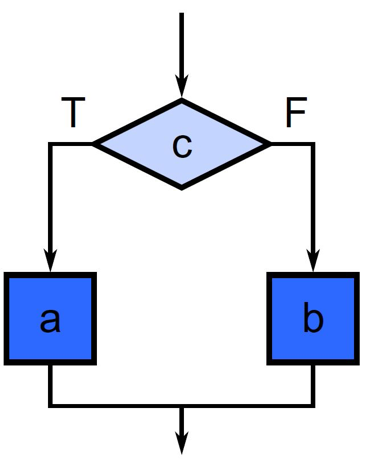
\includegraphics[width=0.3\textwidth]{arrow/select.png}
    \caption{Visualization of the branching pattern \cite{mccoolStructuredParallelPrograming2012}}
    \label{SArrow:fig:select}
\end{figure}

First of all, the branching pattern illustrated by \figref{SArrow:fig:select} is equivalent to an expression formed by \hask{|||} combinators, where the data constructor \hask{Left} leads to one computation path and the data constructor \hask{Right} leads to another computation path. It seems to be a simple pattern but it is useful when composed with other complicated patterns. We will use an example to illustrate at the end of this section.
\begin{figure*}[ht]
    \begin{subfigure}[b]{0.475\textwidth}
       \centering
       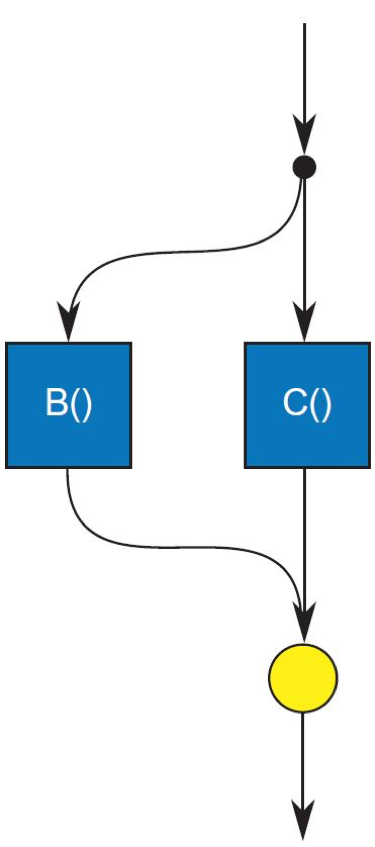
\includegraphics[width=0.60\textwidth]{arrow/fork.png}
        \caption{Visualization of the fork-join pattern \cite{mccoolStructuredParallelPrograming2012}}
        \label{SArrow:fig:fork}
    \end{subfigure}
    \hfill
   \begin{subfigure}[b]{0.475\textwidth}
        \centering
        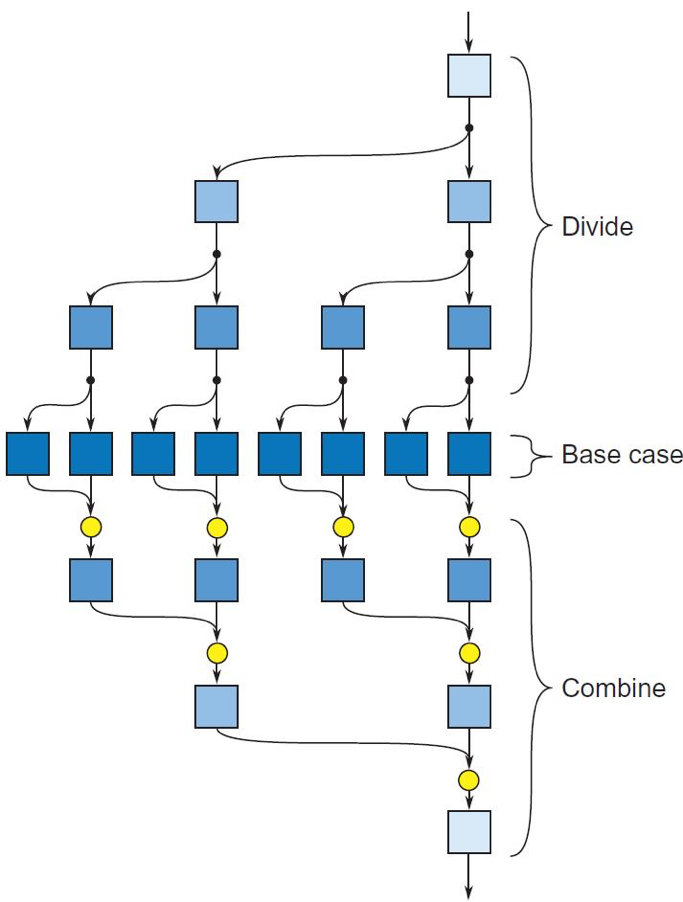
\includegraphics[width=\textwidth]{arrow/dq.png}
        \caption{Fork-Join Pattern for Divide-Conquer \cite{mccoolStructuredParallelPrograming2012}}
        \label{SArrow:fig:dq}
    \end{subfigure}
    \caption{Fork-join pattern and divide-and-conquer algorithms}
\end{figure*}
Secondly, the fundamental building block of parallel pattern, the fork-join pattern illustrated by \figref{SArrow:fig:fork} can be expressed by \hask{&&&} combinator. The SArrow produced by \hask{&&&} has the two-ary tuple as the output type collecting the computation result of the main thread and the forked thread and also acts as a synchronization point.
\begin{figure}[ht]
    \centering
    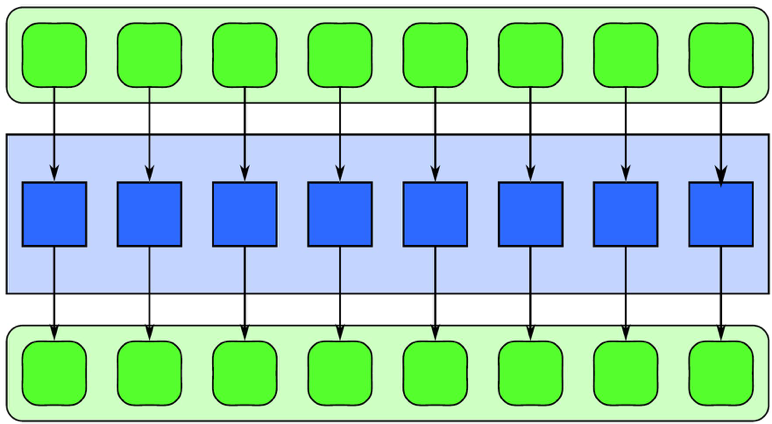
\includegraphics[width=0.5\textwidth]{arrow/pmap.png} 
    \caption{Visualization of parallel map \cite{mccoolStructuredParallelPrograming2012}}
    \label{arrow:fig:pmap}
\end{figure}
\begin{listing}[ht]
    \inputminted{Haskell}{arrow/pmap.hs}
    \caption{Parallel map in SArrow}
    \label{arrow:code:pmap}
\end{listing}
Thirdly, the familiar parallel map pattern illustrated in \figref{arrow:fig:pmap} is also a candidate to be expressed in SArrow. The code sample is in \coref{arrow:code:pmap}. \hask{pmap} splits the input \hask{a} into 4 chunks using the splitting function \hask{s}, applied the elemental function \hask{f} and the arrow combinator \hask{***} in parallel and finally use the collecting function \hask{c} to collect the results. Usually, the input \hask{a} is a list and \hask{s} splits the list into 4 equal chunks. The number of times where function is \hask{f} applied decides the number of ways of parallelism. % We will describe a possible solution to make \hask{pmap} more generic so that we do not need write a new functions for every number of ways of parallelism. (TODO).

\begin{figure}[ht]
    \centering 
    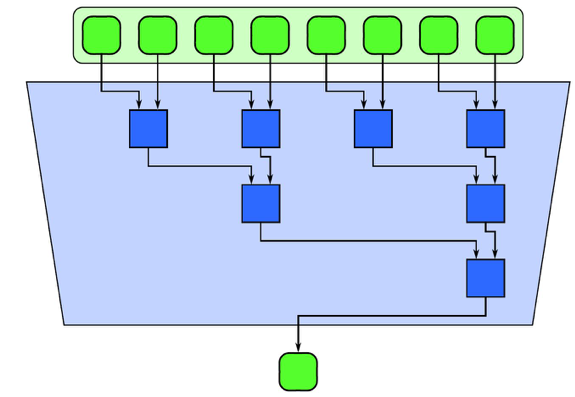
\includegraphics{arrow/preduc.png}
    \caption{Visualization of parallel reduce in SArrow \cite{mccoolStructuredParallelPrograming2012}}
    \label{arrow:fig:preduc}
\end{figure}
\begin{listing}[ht]
    \inputminted{Haskell}{arrow/preduc.hs} 
    \caption{Parallel reduce in SArrow}
    \label{arrow:code:preduc}
\end{listing}
Fourthly, we can apply the similar logic to express parallel reduce pattern shown in \figref{arrow:fig:preduc}. The code sample is in \coref{arrow:code:preduc}. The result of parallel reduce has similar type signature as the collecting function in \hask{pmap} so it is often used with the \hask{pmap} function. We use nested tuple \hask{(a, (a, (a,a)))} to represent a sized array of data. The \hask{helper} function transforms the array representation of data into a form so that we apply the reduce function \hask{r} to the elements pair-wise and parallel.

\begin{listing}[ht]
    \inputminted{Haskell}{arrow/dq.hs}
    \caption{2-ways and 3-levels divided-and-conquer algorithm in SArrow}
    \label{SArrow:dq}
\end{listing}
Finally, more complicated pattern can be expressed compositely from simpler pattern expressed in SArrow. We can use a typical divide-and-conquer algorithms implemented with fork-join as an example. \figref{SArrow:fig:dq} shows a divide-and-conquer algorithms with 2-ways and 3-levels of fork-join. The algorithm can be expressed in SArrow shown in \coref{SArrow:dq}. The divide-and-conquer pattern can be built recursively in Haskell. For the base case, we simply apply the basic computation. Otherwise, we first call split and then call the function recursively with the level decremented by one and, in the end, call the merge to combine the results. Every expressions in the function definition are connected using arrow combinators. A 3-level divided-and-conquer algorithm is constructed by passing 3 to the function resulting a algorithm with $2^3 = 8$-way parallelism.

\begin{figure}[ht]
    \centering
    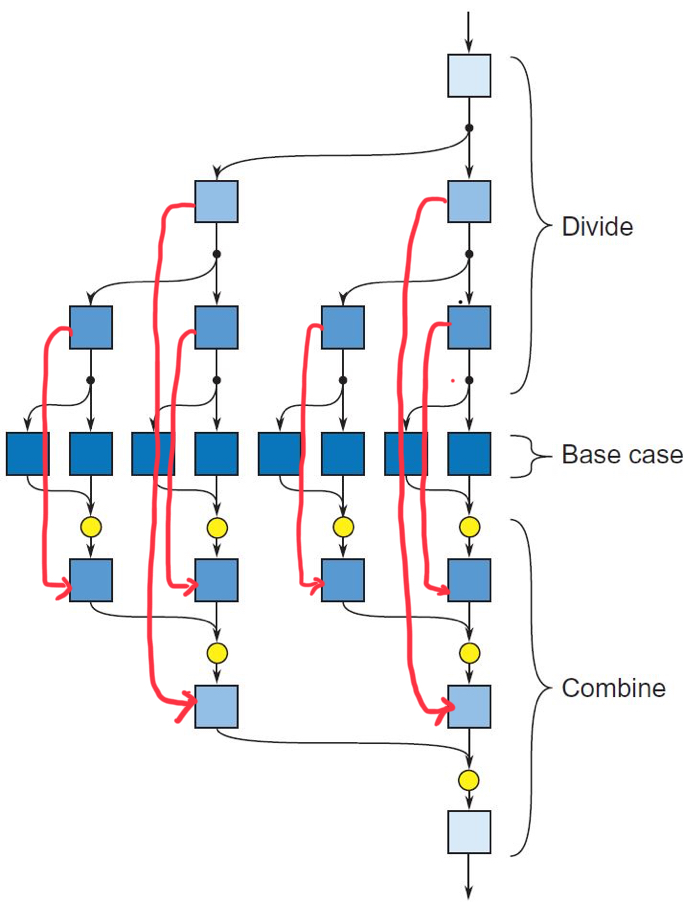
\includegraphics[width=0.5\textwidth]{arrow/dq2.jpeg}
    \caption{Combination of branching pattern and divide-and-conquer pattern}
    \label{SArrow:fig:brdv}
\end{figure}
In addition, the divide-and-conquer parallel pattern can be optimized when combining with branch pattern. The branch pattern allows us to add shortcuts to the pattern (illustrated in the \figref{SArrow:fig:brdv}, redlines represent the alternative computation path provided by branching patterns). The shortcut give us the ability to decide whether to do local computation or split  into multiple subtasks depending on the input size. When the input size is small, the overhead of the latter usually outweighs its parallelism. Adding the simple branching pattern results in a pattern that is adaptive to various input size with better performance.

The implementation demos the power of implementing SArrow as a domain specific language embedded in Haskell. We make full use of Haskell features, i.e high order functions and polymorphic functions to construct expressive, composable and generic computation patterns.

More examples of algorithms formed by SArrow, e.g. dot product or merge sort are shown in the \secref{eval}.
\section{Implementation of arrow combinators} \label{SArrow:impl}
In this chapter, we will present naive implementation and the optimized solution is introduced in the next section.

\begin{listing}[ht]
    \inputminted{Haskell}{arrow/kleisli.hs} 
    \caption{The implementation of arrow instance for Kleisli arrow of a monad}
    \label{arrow:code:kleisli}
\end{listing}
The intuition why SArrow is an instance of Arrow comes from the Kleisli arrow of a monad is an instance of Arrow class (shown in \coref{arrow:code:kleisli}). The \hask{cont} field in the Pipe has similar type signatures as the \hask{runKleisli} field in the Kleisli arrow. From the previous section, we shown that Proc is a monad so Pipe is just an extended version of Kleisli arrow where computations in Pipe usually finish in one of the process stored in \hask{env} instead of finishing at \hask{cont} like Kleisli arrow. Intuitively, SArrow, a function from the role to the Pipe, should be an instance of Arrow since Pipe looks like an arrow instance and functions are composite.

The essential issue when implementing arrow combinators is how to connect one Pipe by another Pipe. The first problem we need to address is how to deal with the \hask{cont} in the tail Pipe. We know that only one \hask{cont} field exists in the resulting Pipe and it must be that from the head Pipe. Hence the only option is to convert it to a Proc expression and store the converted expression in the updated env in the resulting Pipe. A right way to do it bind the cont with the action: receive from end in the first Pipe. Also, extend the proc related to the end in the head Porc with action: send to start in the second Pipe. Besides addition of the converted \hask{cont} expression, the new env is formed by merging the env from the head Pipe and the env from the tail Pipe. Merging two envs is trivial. When there are duplication, we simply use monadic bind to combine them so that the actions belonging to head Pipe followed by the actions belonging to the tail Pipe. The \hask{start} field in the resulting Pipe is the same as that from the head Pipe and the \hask{end} field will be set the same as that from the tail Pipe.
\begin{listing}
\inputminted{Haskell}{arrow/impl.hs}
\caption{The simplified implementation of \hask{>>>}}
\label{SArrow:code:impl}
\end{listing}
We can apply the Pipe composing function to implement arrow combinators for SArrow. The implementation is just apply the first SArrow with the input role (don't forget SArrow is a function) to get the Pipe and apply the second SArrow with a new role to get the second Pipe (usually in order to avoid duplication of roles, the new role is set to be maximum role in the first Pipe + 1) and finally apply the Pipe composing functions to both Pipe. A simplified code explanation can be seen in \coref{SArrow:code:impl}. The rest of combinators can be implemented in a similar fashion.

\section{Strategies for optimized role allocations} \label{SArrow:roleAllc}
From the last section, we know the number of roles in the system is directly related to the number of processes in the final generated code. Hence, role allocating is an essential part in generating efficient parallel programs. 

In this section, we propose strategies for optimizing role allocations. We have two goals in mind when optimizing; The first one is we would like to reduce the number of roles (processes) in the computation since the overhead of thread creation and data transmission has negative impact on performance. The second one is we do not want roles duplication when we try to compose SArrows since role duplications means the different computation must be merged in the same role and computations in the same thread is sequential hence role duplications has negative impact on degree of parallelization. 

If we only put the first goal in mind, an easy solution will be setup an upper bound of the number roles, and then we cycle through a fixed bound when allocating new roles. Processes corresponding to duplicated roles can be simply merged using binds since Proc is a monadic DSL and duality check ensures binding will not cause deadlocks. However, this strategies is not ideal since duplications of roles will decrease the degree of parallelization in the system.

If we only consider the second goal, naive strategies used in the previous section will satisfy the goal. However, the number of channels required and the number of roles in the system will grow exponentially. In a divided-and-conquer algorithm, the number of channels increases from 10 to 120 and the number of roles increases from 6 to 36 when the level is increased from 1 to 3.
\begin{table}[ht]
\begin{displaymath} 
    \inference[id]{x: \text{Role}, \quad a: \text{Type}}{id : \text{SArrow a a}, x \Rightarrow x}
\end{displaymath}
\caption{Role allocation for id}
\label{SArrow:ra:example}
\end{table}

For the purpose of illustration, we use inference rules to explain our proposed strategies for optimized role allocations when composing SArrows. Please see \tabref{SArrow:ra:example} as an example. $x \Rightarrow x$ means the computation start with role $x$ and end with role $x$.
\begin{table}[ht]
\begin{displaymath} 
    \inference[compose]{e1 : \text{SArrow a b}, x \Rightarrow y, \quad e2: \text{SArrow b c}, y \Rightarrow z}{e1 \; \hask{>>>} \; e2 : \text{SArrow a c}, x \Rightarrow z}
\end{displaymath}
\vskip\baselineskip
\begin{displaymath} 
    \inference[arr]{f : \text{Core (a} \rightarrow \text{b)}, \quad x: \text{Role}}{\text{arr } f: \text{SArrow a b}, x \Rightarrow x}
\end{displaymath}
\vskip\baselineskip
\begin{displaymath}
    \inference[arrow choice: \hask{|||}]{e1: \text{SArrow a c}, x \Rightarrow y, \quad e2: \text{SArrow b c}, x \Rightarrow z}{e1 \; \hask{|||}\; e2 : \text{SArrow (Either a b) c}, x \Rightarrow \text{max}(y, z)}
\end{displaymath}
\vskip\baselineskip
\begin{displaymath}
    \inference[arrow choice: \hask{+++}]{e1: \text{SArrow a c}, x \Rightarrow y, \quad e2: \text{SArrow b d}, x \Rightarrow z}{e1 \;\hask{+++}\; e2 : \text{SArrow (Either a b) (Either c d)}, x \Rightarrow \text{max}(y, z)}
\end{displaymath}
\vskip\baselineskip
\begin{displaymath}
    \inference[arrow: \hask{&&&}]{e1: \text{SArrow a b}, x \Rightarrow y, \quad e2: \text{SArrow a c}, (y+1) \Rightarrow z}{e1 \;\hask{&&&}\; e2 : \text{SArrow a (b, c)}, x \Rightarrow z}
\end{displaymath}
\vskip\baselineskip
\begin{displaymath}
    \inference[arrow: \hask{***}]{e1: \text{SArrow a b}, x \Rightarrow y, \quad e2: \text{SArrow a' c}, (y+1) \Rightarrow z}{e1 \;\hask{***}\; e2 : \text{SArrow (a, a') (b, c)}, x \Rightarrow z}
\end{displaymath}
\caption{Rules fo role allocations of different combinators}
\label{SArrow:ra:rule}
\end{table}

The rule for the rest of combinators are shown in \tabref{SArrow:ra:rule}. Notice that for compose, id, arr and ArrowChoice we do not introduce any new roles, in other words, there is no parallelization for these combinators. Reader may find it strange that we do not intent to parallelize arr combinator which lifts a sequential computation represented by Core (a $\rightarrow$ b) into SArrow. It makes sense to introduce a new role to execute the computation and hence parallelize computational heavy tasks. We use this strategy in the first place but later we found a more suitable strategy exists which will be introduced in the later paragraph. Also, another reason not to introduce new role when encountering arr combinators is that we gained function fusion for free. Simple function i.e. fst, inject left or snd are automatically fused into more complicated user defined functions. Introducing new roles for these simple functions will damage performance. % o introduce new roles when encounter \hask{&&&}. In this way, we do not sacrifice any degree of parallelization but keep the number of roles in the system at the minimum. 

For the class of combinators belonging to arrow choice, we do not introduce any new role. The expressions at the lhs and at the rhs starts with the same role $x$ because when only one code path will be executed as the name choice suggested so we should not use separate roles for two expressions that will never be executed simultaneously. In the end, we decided the computation end in the role max$(y,z)$. Max guarantees that there will not be role duplications when we compose expressions formed by ArrowChoice combinators with other combinators. For the implementation, all process in both left and right SArrow expression are wrapped inside a branch operation separately. Assume max$(y, z) = y$, the process at the role $y$ will be extended with actions that receive data from min$(y, z) = z$ role at its right branch. Finally, applying inject left and inject right at left and right branches gives us Either type as the output.

Finally, we discovered the right place to allocate new roles is \hask{&&&} combinator. As shown in type signature, product types mean computation at both branches will both be executed and they are independent. In order to make sure both computation are executed simultaneously, we constraint that the right SArrow expression must start with a role greater than the end role of the left SArrow expression. This ensures no role duplications hence maximize parallelism. The combined expression ends in the end role of the right SArrow expression instead of introducing a unnecessary new role. For the implementations, the process corresponded to end role $z$ are extended with actions that receive data from the end role $y$ of the left process and store the computation of SArrow expression at the right side and finally output a pair.

Even though from the implementation point of view, SArrow composition with the optimized role allocations is ad-hoc and less elegant to implement because we need to consider composition by send-and-receive and composition by local monadic bind and more edge cases to be dealt with compared to the naive solution in the last section where composition is done solely by send-and-receive and role allocations is mindless. We believe the effort is worthy because for a n-level divided-and-conquer algorithms, the optimized role allocation strategies allocate $2^n$ roles in total which is the same as the number of way of parallelization in theory. All the roles are used to maximize parallelism instead of wasting the valuable resources to create roles that merely transmit data.

In conclusion, the optimized strategy presented in this chapter is not the only solution. For example, there is a strategy that only introduce new roles into the computation graph when encountering a specific atomic functions. Different strategies result in different communication structures hence different kind of parallelisms. We should choose the right strategy depending on the specific task.
\section{Satisfaction of arrow laws}
We have provided the implementation of SArrow combinators that is similar to the arrow interface. However, the implementation is not enough to state that SArrow is an arrow interface. Furthermore, we need to prove that SArrow satisfy the arrow laws. Because of the limited context, we will present justification instead of formal proofs. We will focus on arrow laws. The justification for arrow-choice law can be reasoned in a similar way.
\begin{table}[ht]
    \begin{align*}
        arr(Id) >>> a &= a \tag{1}\\
        a >>> arr(Id) &= a \tag{2}\\
        (a >>> b) >>> c &= a >>> (b >>> c) \tag{3}\\
        arr(f;g) &= arr(f) >>> arr(g) \tag{4}\\
        first(a) >>> arr(Fst) &= arr(Fst) >>> a \tag{5}\\
        first(a) >>> arr(\alpha) &= arr(\alpha) >>> first(first(a)) \tag{6}\\
        first(a >>> b) =& first(a) >>> first(b) \tag{7}\\
    \end{align*}
    \caption{Arrow laws \cite{atkeyWhatCategoricalModel2011}}
    \label{arrow:tab:law}
\end{table}

\tabref{arrow:tab:law} shows the rules of arrow laws. We includes a subset of law that contains the \hask{first} combinator. The other half of laws that contains the \hask{second} combinator can be proved by symmetry. \hask{first} combinator is implemented as \hask{first = (*** id)} and $\alpha :: ((x, y), z) -> (x, (y, z))$.
\begin{figure}[ht]
    \centering
    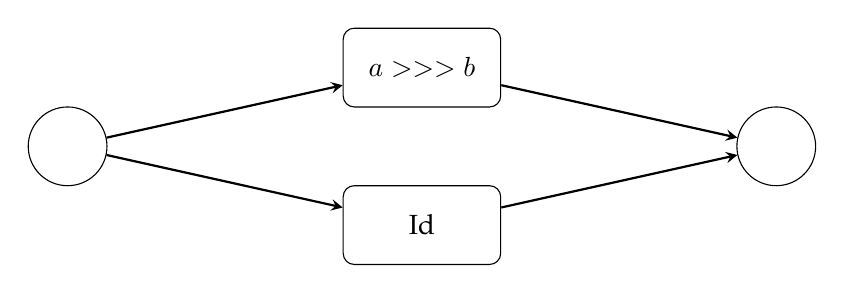
\begin{tikzpicture}[xscale=1.5]
        \tikzstyle{proc} = [rectangle, rounded corners, minimum width=2cm, minimum height=1cm,text centered, draw=black] 
        \tikzstyle{proc1} = [circle,  minimum width=1cm, minimum height=1cm,text centered, draw=black] 
        \tikzstyle{arrow} = [thick,->,>=stealth]
        \node (a) [proc1] at (0, 0) {};
        \node (c) [proc] at (3, 1) {$a >>> b$};
        \node (d) [proc1] at (6, 0) {};
        \node (e) [proc] at (3, -1) {Id};
        \draw[arrow] (a) to (c);
        \draw[arrow] (c) to (d);
        \draw[arrow] (a) to (e);
        \draw[arrow] (e) to (d);
    \end{tikzpicture}
    \vskip\baselineskip
    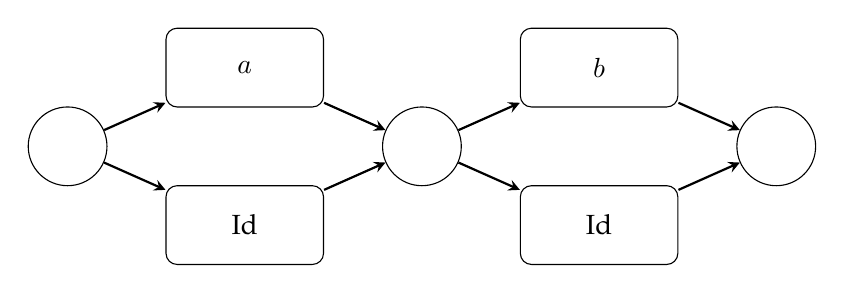
\begin{tikzpicture}[xscale=1.5]
        \tikzstyle{proc} = [rectangle, rounded corners, minimum width=2cm, minimum height=1cm,text centered, draw=black] 
        \tikzstyle{proc1} = [circle,  minimum width=1cm, minimum height=1cm,text centered, draw=black] 
        \tikzstyle{arrow} = [thick,->,>=stealth]
        \node (a) [proc1] at (0, 0) {};
        \node (c) [proc] at (1.5, 1) {$a$};
        \node (d) [proc1] at (3, 0) {};
        \node (e) [proc] at (1.5, -1) {Id};
        \node (f) [proc] at (4.5, 1) {$b$};
        \node (g) [proc] at (4.5, -1) {Id};
        \node (h) [proc1] at (6, 0) {};
        \draw[arrow] (a) to (c);
        \draw[arrow] (c) to (d);
        \draw[arrow] (a) to (e);
        \draw[arrow] (e) to (d);
        \draw[arrow] (d) to (f);
        \draw[arrow] (d) to (g);
        \draw[arrow] (f) to (h);
        \draw[arrow] (g) to (h);
    \end{tikzpicture}
    \caption{Graphical representation of equation (7)}
    \label{arrow:fig:eq7}
\end{figure}

\begin{figure}[ht]
    \centering
    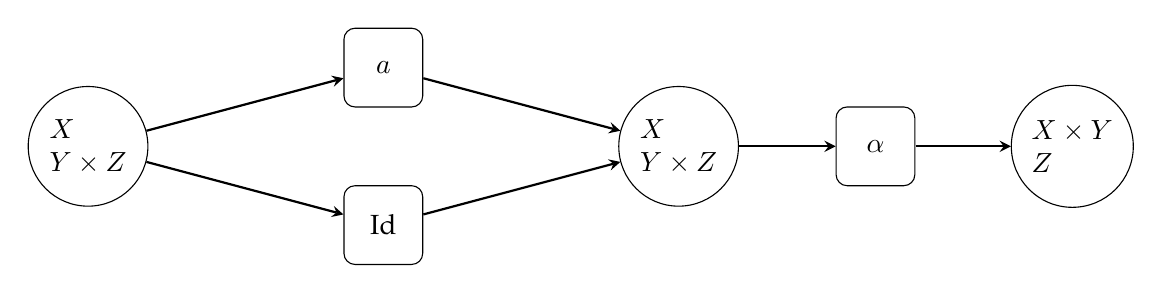
\begin{tikzpicture}[xscale=2.5]
        \tikzstyle{proc} = [rectangle, rounded corners, minimum width=1cm, minimum height=1cm,text centered, draw=black] 
        \tikzstyle{proc1} = [circle,  minimum width=1cm, minimum height=1cm,text centered, draw=black] 
        \tikzstyle{arrow} = [thick,->,>=stealth]
        \node [proc1, align=left] (2) at (0, 0) {$X$ \\ $Y \times Z$};
	 \node [proc] (3) at (1.5, 1) {$a$};
	 \node [proc] (4) at (1.5, -1) {Id};
	 \node [proc] (7) at (4, 0) {$\alpha$};
	 \node [proc1, align=left] (8) at (5, 0) {$X \times Y$ \\ $Z$};
	 \node [proc1, align=left] (9) at (3, 0) {$X$ \\ $Y \times Z$};
     \draw[arrow] (2) to (3);
     \draw[arrow] (3) to (9);
     \draw[arrow] (2) to (4);
     \draw[arrow] (4) to (9);
     \draw[arrow] (9) to (7);
     \draw[arrow] (7) to (8);
    \end{tikzpicture}
    \vskip\baselineskip
    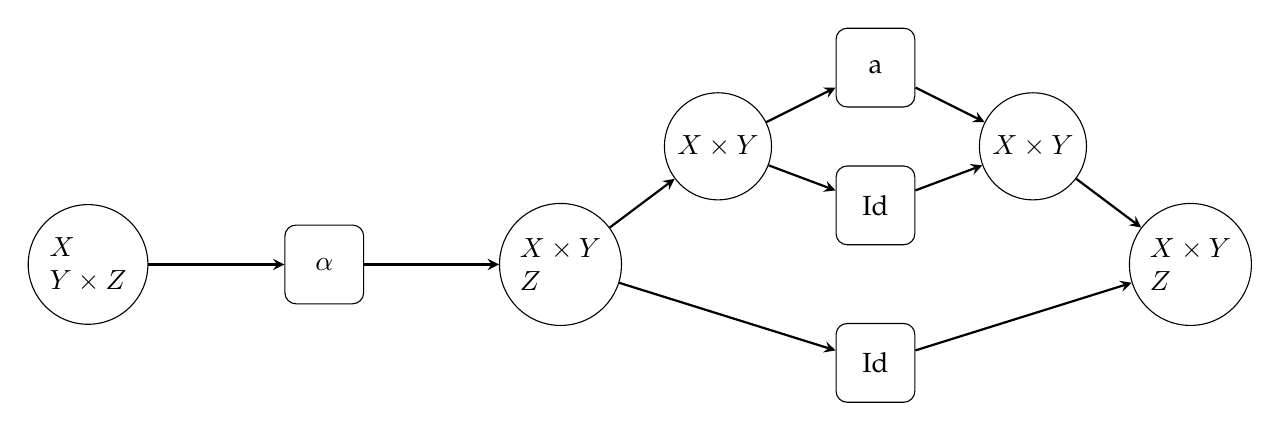
\begin{tikzpicture}[xscale=2.0]
        \tikzstyle{proc} = [rectangle, rounded corners, minimum width=1cm, minimum height=1cm,text centered, draw=black] 
        \tikzstyle{proc1} = [circle,  minimum width=1cm, minimum height=1cm,text centered, draw=black] 
        \tikzstyle{arrow} = [thick,->,>=stealth]
		\node [proc1, align=left] (0) at (-1, 0) {$X$ \\ $Y \times Z$};
		\node [proc] (1) at (0.5, 0) {$\alpha$};
		\node [proc1, align=left] (2) at (2, 0) {$X \times Y$ \\ $Z$};
		\node [proc] (5) at (4, 2.5) {a};
		\node [proc] (6) at (4, 0.75) {Id};
		\node [proc1] (7) at (5, 1.5) {$X \times Y$};
		\node [proc1, align=left] (8) at (6, 0) {$X \times Y$ \\ $Z$};
		\node [proc1] (9) at (3, 1.5) {$X \times Y$};
		\node [proc] (10) at (4, -1.25) {Id};
		\draw[arrow] (0) to (1);
		\draw[arrow] (1) to (2);
		\draw[arrow] (2) to (9);
		\draw[arrow] (9) to (5);
		\draw[arrow] (9) to (6);
		\draw[arrow] (5) to (7);
		\draw[arrow] (6) to (7);
		\draw[arrow] (7) to (8);
		\draw[arrow] (2) to (10);
        \draw[arrow] (10) to (8);
    \end{tikzpicture}
    \caption{Graphical representation of equation (6)}
    \label{arrow:fig:eq6}
\end{figure}

We argue above equation holds if both sides of equation express the same computation. Equation (1), (2) holds because lifting Id from Core to SArrow will not modify the result of computation due to the semantics of Id. Equation (3) is the associativity rule of $>>>$. Left side of the equation sends the output from $a >>> b$ to the input of $c$ while right side sends the output of $a$ to the input $b >>> c$. The communication structure might change but they both represents the same computation. Equation (4) is valid because applying the input value to composition of f;g is the same as applying the input to f followed by a message passing (data communication could be local which means the communication structure for both side of equations are the same in this case) and then applying it to g. One might claim that the left side is more efficient than the right side due to the fusion depending on the role allocation strategy. Equation (5) holds because they both represents a computation that take a pair input and apply the function a to its first position and return the result. Right hand side of equation (7) represents a SArrow expression that applies a on left position of input pair and applies Id on the right position of input pair in parallel, collects the results and applies b on left position of input pair and applies Id on the right position of input pair while left side fused a and b together and apply them in one step hence there is only one join point. \figref{arrow:fig:eq7} is a graphical representation of equation (7). Obviously they represents the same computation. We can also derive equation (6) from its Visualization (see in \figref{arrow:fig:eq6}).

\section{Conclusions}
Arrow interface is the perfect interface to express general computation for this project because not only is it intuitive to understand and visualize but also its combinators \hask{***} and \hask{&&&} has built-in parallel natural.

So far, we've used SArrow to help us compile Par-Alg to SPar. The remained challenge is the code generation from SPar to a target platform. In the next chapter, we will introduce our methods for code generation and specifically code generation to C. Once we achieved this, every computation in SArrow can be transformed into parallel C code in one step.

% \section{Applications}
% \subsection{Hassle-free compilation from ParAlg to SArrow} %Hassle-free
% \subsection{An interface for arrow computation with automatic parallelization}
% \section{Power of arrow and EDSL: &)expressibility and composability}
% \subsection{Arrow interface}
% \subsection{Haskell as the host language}
\chapter{Type-safe code generation from SPar} \label{chap:cg}
SPar has two components: Core representing the unit of computation and Proc as a skeleton of the computation, describing the communication patterns. Naturally, the process of code generation from SPar should be divided into two parts correspondingly. We choose to make two parts independent of each other so that it's possible to swap the code generation strategy of one component without modifying another one.

The procedure of code generation is standard: transformation. We start our programs in a high level DSL and run a series of transformation to low-level DSL. SPar expressions are converted to a low-level EDSL which is then transformed to an abstract syntax tree (AST) of C (TODO cite the package). The generated code is obtained by pretty printing the AST.
\section{Instr: A low-level EDSL for channel communication}
In Proc, we have high-level actions like select, broadcast and branch abstracting implementation details, i.e variable declaration, variable assignment, channel initialization, channel communication and channel deletion. Hence, we need to define a EDSL containing instructions related to these low-level operations. We name it Instr. A Spar programs will be translated to a sequence of Instr. 

When we design Instr, we keep the simplicity in mind so Instr is not coupled with any fancy language feature related to some specific target languages. Any reasonable target language with a channel communication library can be easily converted from Instr.
\subsection{Syntax and semantic}
\begin{listing}
    \inputminted{Haskell}{codegen/instr.hs} 
    \caption{The syntax of Instr in Haskell with accompanying low-level data types}
    \label{codegen:code:instr}
\end{listing}
The definition of Instr is seen in \coref{codegen:code:instr}. \hask{Channel} is our abstract representation of Channel in Instr. It is indexed by a type a from the reified type \hask{ReprType a}. More details of this reified type will be introduced in \secref{codegen:sec:repr}. This type parameter preserves type in channel initialization hence make sure the value to be sent or received in this channel has the same type as this channel. This is necessary because for some target languages, the channel are typed. Similarly, type parameters in \hask{Exp} have the same functionality. \hask{Exp} is just a wrapper of the expression in Core. In later stages, we will take care of code generation of \hask{Exp} along with \hask{Instr}. \hask{Instr} defines the set of statements that will be generated and \hask{Exp} represents the sequential computation, which is a value that will be generated.

The semantic of Instr operations are similar to what their names suggest. \hask{CInitChan} represents operations that initialize a channel according to the given type and cid. \linebreak \hask{CDeleteChan} will destroy a channel. \hask{CSend} operation sends the value \hask{Exp a} through the Channel. \hask{CRecv} action means the value received in the channel will be assigned to variable whose postfix name is the int field. \hask{CEnd} means the instruction exits with the value \hask{Exp a}. \hask{CDecla} and \hask{CAssgn} are instructions for variable declaration and assignment. The type of the variable is determined by \hask{ReprType a} and the value is \hask{Exp a}. \hask{CBranch} and \hask{CSelect} are used to express conditional control flow of the Instr languages. SPar action like broadcast are built on top of these operations. For \hask{CBranch}, the first field represents the value of Either type to be received via the channel and two \hask{Seq Instr}s represents the sequence of \hask{Instr}s in the left branch and the right branch. For \hask{CSelect}, the first field represents the variable containing Either value and the second field field represents the variable whose value is assigned by the end results of instructions from either the left branch or the right branch. The third and fourth fields represent the instructions in the left branch and the right branch.

\subsection{Representation types} \label{codegen:sec:repr}
SPar programs cannot be fully parametric since the target languages of code generation from SPar are usually less expressive, i.e, they do not treat function type \hask{a->b} as a value, and are less efficient when processing with some specific form of data, i.e, languages targeting GPUs are usually more productive in dealing with array of floating point number while slow in working with aggregate structures \cite{mcdonellTypesafeRuntimeCode}. 
\begin{listing}
    \inputminted{Haskell}{codegen/repr.hs}    
    \caption{The definition of representation types}
    \label{codegen:code:repr}
\end{listing}
\begin{listing}
    \inputminted{Haskell}{codegen/const.hs} 
    \caption{An example usage of reified type in the code generation}
    \label{codegen:code:const}
\end{listing}
Hence, we need to restrict the set of types allowed in SPar. We achieve this using the type class \hask{Repr} and corresponding reified type \hask{ReprType} (shown in \coref{codegen:code:repr}). \hask{Repr} determines the set of type allow in SPar. Reified type \hask{ReprType} will be used to alter the behaviors of code generation based on the type. This can be simply done by pattern matching because reified types are values in Haskell \cite{ReifiedTypeHaskellWiki}. To be more concrete, \coref{codegen:code:const} gives a demo. \hask{constToCExpr} is function that handle code generation from constant value to expression in C programming languages. By pattern matching, we vary the behaviors of code generation so that constants with different types has their own way to be represented in C.

In conclusion, we allow the following type: numerical type like \hask{Float} and \hask{Int}, the unit type \hask{()}, the label type which is used in the code generation of select and branch and the aggregate type: list, product and sum that are built recursively, to be expressed in SPar.

\section{Compilation from SPar to Instr}
% \subsection{Two stages of compilation}
\subsection{Transformation from Proc to Instr}
As described in the previous section, Instr contains a data type called \hask{Exp} which is a wrapper of Core expression. Compiling Core to Instr is hence not difficult. The challenge of compiling Core is mainly how to compile it to a specific target language. This will be discussed in the next subsection.  

In this section, we will explain how we transform operations in Proc to Instr. Generally speaking, each Proc operation is mapped to a sequence of actions in Instr. The transformation algorithm from a Proc expression to a sequence of Instr can be implemented easily by traversing Proc expression, applying the mapping and collecting the results by concatenation. This is an advantage of using free monad technique to build the AST because Proc expression can be treated as a data structures and traversing recursive data structures can be easily done in Haskell. In addition, operations like \hask{Recv} which involves continuation whose type is \hask{Core a -> next} in their constructors are treated differently than those operations whose constructors only have a value type \hask{next}. The latter is easy to implement, we can simply call the traversing function recursively. For the former, we have to pass an expression whose type is \hask{Core a} to the continuation so that we can recursively call the traverse function recursively on the results of applying value to the continuation. The answer to what Core expression should be used is \hask{Var} denoting variable. Passing a unique variable to the continuation gives us \hask{next} inexpensively and we will define where does values of variables comes from for each operations in Proc. 

We have introduced the general principle to the readers. Now let us dig into details of translation rules for each operations. 

\begin{itemize}
    \item \textbf{Pure. } It is the base case in free monad. Hence it is mapped to the \hask{CEnd} instruction.
    \item \textbf{Send. } It is mapped to a sequence of three instructions. First of all, We declared a temporary variable using \hask{CDecla} and then assign the value that will be sent to this variable using \hask{CAssgn} and send the content of the variable via the specific channel. The problem of how make sure the same channel is used in a send-and-receive pair will be discussed in the next sub chapter.
    \item \textbf{Recv. } It is the reverse of send operation. Firstly, it declares a new variable with \hask{CDecla} and use \hask{CRecv} to assign the value received from the sender to this variable. Notice that the recv has a continuation, we will pass the variable declared in the first instr to the continuation to traverse the Proc expression recursively as discussed above. 
    \item \textbf{Select. } It is a more complicated operations. Its constructor contains two continuation: one for left branch and one for right branch. Hence for this instruction, we need to declared two variable to passed into continuations. The value of both variables is assigned by the Core expression whose value is a Either type. Besides, we need to send label indicating whether the execution of the left branch or the right branch of the receiver is selected. Its value is assigned by the either value as well and the sending operation is done by \hask{CSend}. Finally, we call the transforming function recursively on the left branch and right branch and combine the results using \hask{CSelect}.
    \item \textbf{Broadcast. } The mapping from Broadcast is similar to that of Select. The only difference is that the former sends to a list of receivers while the latter sends to a single receiver. So in this operation, we will have multiple \hask{CSend} corresponding to each receiver.  
    \item \textbf{Branch. } It is the reverse of the Select operation. So it will use \hask{CRecv} to receive a label from the sender and call recursively on two branches and finally use \hask{CBranch} to collect results.
\end{itemize}
\subsection{Strategies for channel allocations}
Channel allocations is important because correction allocation is essential in making sure the correctness and deadlock-free of generated code. Besides correctness concerns, we are also want to reduce the amount of channels creations hence increase performances. 

In the first iteration, inspired by the linearity of channels in the $\pi$ calculus, we choose to allocate a one-time channel for each send-and-receive pair. All channels' buffer size is one because of the linearity. Send action will initialize a channel and Receive action will destroy this channel once it receive the value. We use the ensure the same channel is used for the pair. During the transformation, we use a map of queue whose key is a pair of sender id  and receiver id. When visiting the send action, it will push the channel into the queue and the corresponding received operation will pop the channel from the queue. Because we've ensured the duality of all processes in the system, we can claim the channel is right for each send-and-receiver pair. However, we realize this strategy is complicate to implement and not resource efficient since too many channels are initialized.

In the second iteration, we come up with a more efficient and simple strategy. The buffer size of all channels is still one due to the same reason about linearity. However, we decide to only allocate one channel for a pair of sender and receiver. We will not destroy the channel after the value has received and will reuse the channel for the next communication. When all processes have returned, we will destroy all channels at once. For this strategy, we have simplified the state from a map of queues of channels to a map of channels.
% \subsection{Type preservation}
\subsection{Monad for code generation}
\begin{listing}[ht]
    \inputminted{Haskell}{codegen/monad.hs} 
    \caption{States required during the traversal}
    \label{codegen:code:monad}
\end{listing}
From the last two subsections, we need to maintain a number of states during the compilation process. Hence we define a state monad to be used during the traversal. The \hask{CodeGenState} is the collection of states with different purposes and it is shown in \coref{codegen:code:monad}. \hask{chanTable} is the map we required during the channel allocation. \hask{varNext} represents the next variable id to used. It will increment by one every time we declare a new variable. It helps us make sure the variable names are unique. \hask{chanNext} has the similar functionality ensuring the uniqueness of channel names. \hask{dataStructCollect} is the set of compound type we encounter during the traversal. With this states, we know what kind of data structures whose definitions will be generated before the generation of executing code.

\section{Code generation to C: from Instr to C}
The last piece of jigsaw is compilation from a sequence of Instr to C. This process is rather simple but trivial. This is simply done by transforming the sequence of Instr to a C AST. We used an open source library: language-c \cite{LanguagecAnalysisGeneration} to represent C AST in Haskell and pretty printing the C AST gives us the generated code. This method can be generalized to any target language. As for the implementation of channel communication in C, we used another open source library: chan \cite{treatPureImplementationGo2019} whose internal is based on shared memory. In the following subsections, we will present some design choices during this final step.
\subsection{Representations of Core data type in C}
\begin{listing}[ht]
    \inputminted{C}{codegen/data.c} 
    \caption{Compound data type in C}
    \label{codegen:code:data}
\end{listing}
The first challenge we face is how to represent data structure in C. For primitive data type like Int or Float, a simple one-to-one mapping is sufficed. It is hard to deal with compound data type in C. First of all, C does not support polymorphic type. Hence, we choose to generate specific data type for every different compound data type even though they have the same structure. We have a way to name the generated data type to avoid name duplication. The naming simply reflects the structure of the data types with its elemental type. For example, \hask{(Int, (Int, ()))} is converted to Prod-Int-Prod-Int-Unit and \hask{Either (Either () (Int, Int)) (Int, Int)} is convert to Sum-Sum-unit-Prod-int-int-Prod-int-int. In this project, all compound types are formed by sum type and product type. The product type will be converted to a struct with two field in C. The sum type is represented by the tagged union type. Tagged union is a struct with two field. The value of the first field indicates whether it is a left value or right value and the value of second field is a union type containing either the left value or right value. We also implement a sorting algorithm based on the depth of compound type so that all necessary data types have been defined before the definition of the compound types. An example of what \hask{Either Int (Int, Int)} will be converted to is shown in \coref{codegen:code:data}.

Another challenge is representation of the recursive type. From the type theory, we learn that a list of int can be expressed as $\mu a. () + \text{Int} \times a$. We might reuse the idea from the last paragraph to generated recursive type in terms of sum and product type. Hence a list of Int will look like the code below.
\begin{minted}{C}
typedef struct Sum_unit_Prod_int_a {
    Label label;
    union {
        int left;
        Sum_unit_Prod_int_a *right;
    } value;
} Sum_unit_Prod_int_a
\end{minted}
However, we believe expressing typical recursive data structures like list of int in this way is bad for performances. Obviously, C has a more efficient way to represent list of int using an array. So we decided to has two ways to represent recursive data structures. For a set of specific recursive data structure, users can write their own representation to exploit the advantages of the target language. For example, a list of int are encoded in C using a wrapper of pointer type (shown in \coref{codegen:code:list}). This way is not very generic but friendly for performances. For other types of recursive data structures where user do not specify their optimized versions in C, we simply apply the method in the last paragraph to encode them in C. This way is generic but not efficient.
\begin{listing}[ht]
\begin{minted}{C}
typedef struct List_int {
        size_t size; int * value;
    } List_int;
\end{minted}
\caption{Optimized represent of List in C}
\label{codegen:code:list}
\end{listing}
\subsection{Compiling from Core to C} \label{codegen:sec:core}
\begin{table}[ht]
    \begin{minipage}{.45\textwidth}
        \begin{displaymath}
            \inference[Var]{}{\toc{\text{Var n}} = \text{vn}} 
        \end{displaymath}
    \end{minipage}
    \hfill
    \begin{minipage}{.45\textwidth}
        \begin{displaymath}
            \inference[Lit]{}{\toc{\text{Lit val}} = \text{toC}(\text{val})}
        \end{displaymath}
    \end{minipage}
    \vskip\baselineskip
    \begin{minipage}{.45\textwidth}
    \begin{displaymath}
        \inference[Fst]{\toc{\text{a}} = c}{\toc{\text{Fst `ap` a}} = c.\text{fst}}        
    \end{displaymath}
    \end{minipage}
    \hfill
    \begin{minipage}{.45\textwidth}
    \begin{displaymath}
        \inference[Snd]{\toc{\text{a}} = c}{\toc{\text{Snd `ap` a}} = c.\text{snd}}        
    \end{displaymath}
    \end{minipage}
    \vskip\baselineskip
    \begin{minipage}{.45\textwidth}
    \begin{displaymath}
        \inference[Inl]{\toc{\text{a}} = c}{\toc{\text{Inl `ap` a}} = \{\text{LEFT}, c\}}
    \end{displaymath}
    \end{minipage}
    \hfill
    \begin{minipage}{.45\textwidth}
    \begin{displaymath}
        \inference[Inr]{\toc{\text{a}} = c}{\toc{\text{Inr `ap` a}} = \{\text{RIGHT}, c\}}
    \end{displaymath}
    \end{minipage}
    \vskip\baselineskip
    \begin{displaymath}
        \inference[Pair]{\toc{\text{a}} = c_1, \quad \toc{\text{b}} = c_2}{\toc{\text{Pair a b}} = \{c_1, c_2\}}
    \end{displaymath}
    \vskip\baselineskip
    \begin{minipage}{.45\textwidth}
    \begin{displaymath}
        \inference[Id]{\toc{\text{a}} = c}{\toc{\text{Id `ap` a}} = c}
    \end{displaymath}
    \end{minipage}
    \hfill
    \begin{minipage}{.45\textwidth}
    \begin{displaymath}
        \inference[Const]{\toc{\text{a}} = c, \quad \toc{\text{v}} = b}{\toc{\text{(Const v) `ap` a}} = b}
    \end{displaymath}
    \end{minipage}
    \vskip\baselineskip
    \begin{displaymath}
        \inference[Prim]{\toc{\text{a}} = c}{\toc{\text{(Prim fname fimpl) `ap' a}} = \text{fname}(c)} 
    \end{displaymath}
    \caption{Rules for compilation from Core to C}
    \label{codegen:rule}
\end{table}
Core has a concise syntax so it does not require too much work to write a function that generate C expressions from Core expressions. Not surprisingly, the compilation is a traversal of the Core expression. Pattern matching on the structure of the core expression alters the behaviors of compilation. \hask{ap} (apply) constructor is used with an expression whose type is \hask{Core (a -> b)} and another expression whose type is \hask{Core b}. The code generation for \hask{ap} depends on the what the function expression is. The code generation rule is explained by the inference rules shown in \tabref{codegen:rule}. $\toc{a}$ means the C code generated by Core expression \hask{a}. $\text{toC}$ is function that convert constant value in Haskell to constant value in C. 
\begin{itemize}
    \item \textbf{Var, Lit:} Code generation of Lit simply convert Haskell value to its corresponding C value. As for Var, it will be converted to a string literal composed of the variable identity prefixed by 'v'.
    \item \textbf{Fst, Inl, Pair\dots} For Inl and Inr and Pair, we used C99 style to initialize struct and union. The rule for generating corresponding struct are explained in the previous subsection. For Fst and Snd, we simply access the specific value using the designator.
    \item \textbf{Id, Const v:} Code generation of Id constructor is same as the code generation of the argument of the Id. Code generation of Const ignores the argument and use code generation of v expression instead.
    \item \textbf{Prim:} Prim constructor represents user defined functions. The code generation for function call of Prim is converted to function call by the name of the primitive function. Users can implement those functions in C and include them in the main generated file.
\end{itemize}

\subsection{The structure of generated C code} \label{codegen:sec:structure}
We have covered the code generation algorithm for each process. We will now tackle how the generated code is structured from a group of interacting processes representing a parallel computation. For each process, we will generate its own C functions that take no argument. We decide to generate an addition C function since function is portable and acts like a black box hiding all the execution details so users can interact with generated code by calling the function. This function will take a parameter as input data and return the computation result. Inside, the function, it will spawn the same number of threads as the number of roles in the system. Each thread will execute the code which is generated from their corresponding Proc expression. In addition to that, the function will send the input parameter to the starting role in the group of Proc to kick off the computation using channel and waiting for the the ending role to send back the computation results. After it receive the result and all the threads have returned, it will return the result. We called this function \hask{proc0}.
\begin{listing}
    \inputminted{C}{codegen/total.c} 
    \caption{An example of generated code}
    \label{codegen:code:total}
\end{listing}

An example of the generated code is shown in \coref{codegen:code:total}. The code contains one process which received a list of int from \hask{proc0}, sort the input by an user defined function and then send the result to \hask{proc0}. We omit global channels declarations and data type declaration for simplicity. 

\section{Conclusion}
With the completion of code generation, we deliver the results we promised in the introduction section. We have implemented a end-to-end process that will generate low-level deadlock-free parallel code from an expressive high-level languages embedded with a flexible backend that can target multiple languages with ease. Now, it is time to evaluate the performances of our achievement with quantitative measurements.
% \subsubsection{Data type in C}
% \subsection{Optimization for common recursive data types in C}
% \subsection{Memory management}

% \chapter{Evaluation}
Beside completing objectives and the project plan defined in the last section, We proposed to evaluate our approach in many parallel algorithms. For example, we will implement mergesort, Cooley-Tukey FFT or N-Body simulations. We will measure the performance against sequential implementations as well as similar algorithms in other parallel frameworks. 

Also, not only will we benchmark the performance of execution of generated code, but also we will benchmark the performance of the tool-chain; \eg measure the compile time against different input sizes. 

Finally, we will focus on measuring the quality of generated code regarding generated code size or readability. We hope we will not experience an exponential growth of code size against input data.
\chapter{Parallel algorithms and evaluation} \label{eval}
\section{Parallelized algorithms}
\subsection{Merge sort}
\subsection{Quick sort}
\section{Benchmarks}
\subsection{Benchmarks against generated Haskell code}
\subsection{Benchmarks against C implementation}
\section{Evaluation}
\subsection{Design choices: Why Haskell?}

\chapter{Conclusions and future work}
% \section{Visualization of the compilation process}
% \section{Design choices}
% \subsection{Why Haskell?}
\section{Future work}
% \chapter{Conclusions and future works}
\section{Conclusions}

Our goal was to implement a backend for code generation for Alg parallel language using a session-typed intermediate language. We not only achieved this but also developed a high-level framework for parallel computation. The project evolved when we tried to fill the huge gap between Alg computation and SPar communication. It was then we started to design an interface as an abstraction layer on top of SPar for ease of compilation from the high-level language to it. The interface iterated from simple helper functions to arrow interface capturing general computation. Then we realized SArrow should not be limited as a compiler writer tool that hides from users, and it should be exposed to users to express computation. The application as a backend is just a side-product while the project shines as a stand-alone framework for parallel code generation.

Iterations of the project lead to the current work: A framework that generates parallel C code along with local types describing the communication patterns by interpreting data-flow as communication, from Arrow based high-level expressions that can be easily formed, composed and manipulated by users with the help of the host language: Haskell. We developed SPar: a session-typed free monad EDSL for message-passing concurrency (see in \charef{chap:spar}) as our intermediate language. Also, we developed tools like local type inferrer to help us reason about the underlying communication structure with external tools from a set of SPar expressions and a simulator to aid experimenting and act as a reference of semantics (see in \charef{chap:impl}). On top of this, we draw inspirations from the Arrow interface and developed SArrow: an interface for writing SPar expressions (see in \charef{chap:arrow}) to form complex computation patterns such as parallel divided-and-conquer and parallel map in a composite way. Finally, we made a code generation backend from SPar to C (see in \charef{chap:cg}). Our benchmark (see in \charef{chap:eval}) shows that our framework can generate efficient parallel code and gain a notable performance boost compared to the sequential code.

In conclusion, with the recent release of AMD's latest generation of consumer CPUs featuring a processor with sixteen physical cores, Moore's law will be replaced by the addition of cores. No need to mention the area of high-performance computing where CPU with 64 cores are common. In contrast, most of the programmers have only written sequential code, and most of the algorithms about which students learn are not parallel. We hope this project can contribute its force on parallelism on CPUs, encouraging more and more programmer to take advantages of modern computing architectures.
\section{Future work}
There are many interesting future works that we would like to implement. We will select some of them to introduce:
\begin{itemize}
    \item \textbf{Optimization for benchmark.} Because of the time constraints, there are lots of space to optimize the generated code. We should do more fine-grained profiling on the generated code. It is interesting to use tools like EzTrace to trace and visualize the execution of all the threads. More importantly, reducing the size of the generated code by eliminating common sub-expressions will be useful. At the moment, there is much code duplication for communication among different roles. The only difference is that the role of participating in the communication. The size of generated code can be reduced a lot if we can extract the common part to a function parameterized by the roles participating. 
    \item \textbf{Integrated user experience.} As demonstrated in the evaluation chapter, users need to write the computation using the EDSL in Haskell and then generate C code. From then on, they need to finish the implementation of their atom functions in C. Finally, they can run the generated code with their data in C. The user experience is isolated when you have to write Haskell first and manually completed the generated code and run them in C. Instead, it will be great if we can provide an integrated user experience where the user does everything in Haskell from writing the high-level expression to collect computation results. This is possible thanks to packages like inline-C and foreign language interface in Haskell. User experience will be greatly improve if we can offer an interface in Haskell that looks like \hask{run :: SArrow a b -> (a -> b)}. This function will take a SArrow expression and produces a function that will convert a Haskell value into C data and execute the computation in C and copy back the C output by foreign language interface to Haskell. From the user pointer of way, it can be used the same as a normal Haskell function with type \hask{a -> b}. Forming a closed loop in Haskell would give us the best user interface and automate a large amount of boilerplate work.
    \item \textbf{Fine-grained control for strategies in role allocation.} We talked about how different role allocation strategies give us different parallel computation. It will be great if we parameterize the SArrow with role allocation strategies and adding ways to specify what strategy will be used at a different stage of the computation. This also opens the possibility for users to implement their strategies to customize their parallel computation tasks.
    \item \textbf{More customizations. } Similar to customized role allocation strategies, we can even have customized representation of sequential computation since the separation of the communication EDSL and the sequential computation EDSL. This can be done by parameterizing \hask{Core} in \hask{Proc}. This kind of work requires well-designed interfaces.
\end{itemize}
% \appendix
\chapter{Examples of generated code} \label{chap:egc}
\section{Merge sort}
\section{Dot product}


\bibliographystyle{ieeetr}
\bibliography{bibs/main}

\end{document}